% !TEX program = xelatex

\RequirePackage{fix-cm}
\documentclass[aspectratio=169,10pt]{beamer}


\def\combineddeck{}

% ======================================================================
%  preamble.tex -- shared by part1.tex, part2.tex, part3.tex
%  A* Search Algorithm -- CSE200, CSE BUET
%  ENGINE: XeLaTeX only (fontspec + OpenType)
% ======================================================================

\usetheme{default}
\useinnertheme{rounded}
\setbeamertemplate{navigation symbols}{}
\setbeamercovered{invisible}

% ----------------------------------------------------------------------
%  1.  FONTS
%      text  -> beamer default  (Latin Modern Sans, beamer's own face)
%      diag  -> Latin Modern Roman  (the LaTeX default face)
%      alg   -> Latin Modern Roman  (the LaTeX default face)
%      math  -> beamer default, untouched
%
%      >>> IBM PLEX SANS: to bring it back as the text font, uncomment
%      >>> the two \set...font lines below.  (TeX Live `plex' fonts,
%      >>> found via kpathsea -- nothing has to live in fonts/.)
% ----------------------------------------------------------------------
\usepackage{fontspec}
% \setmainfont{IBMPlexSans}[Extension=.otf,
%   UprightFont=*-Regular, BoldFont=*-Bold,
%   ItalicFont=*-Italic,   BoldItalicFont=*-BoldItalic]
% \setsansfont{IBMPlexSans}[Extension=.otf,
%   UprightFont=*-Regular, BoldFont=*-Bold,
%   ItalicFont=*-Italic,   BoldItalicFont=*-BoldItalic]
\newfontfamily\diagfont{lmroman10-}[Extension=.otf,
  UprightFont=*regular, BoldFont=*bold,
  ItalicFont=*italic,   BoldItalicFont=*bolditalic]
\let\algfont\diagfont

\usepackage{amsmath,amssymb,mathtools}
\usepackage{booktabs}
\usepackage{pifont}                % \ding symbols (part 2)
\usepackage[table]{xcolor}
\usepackage{graphicx}
\usepackage{tikz}
\usetikzlibrary{arrows.meta,positioning,decorations.pathreplacing,calc,
                shapes.geometric,backgrounds,fit,shadows.blur, tikzmark}

% ----------------------------------------------------------------------
%  2.  PALETTE
% ----------------------------------------------------------------------
\definecolor{rblue}{HTML}{2E2E9C}
\definecolor{rbluedk}{HTML}{1C1C6B}
\definecolor{rbluemd}{HTML}{5A5AC4}
\definecolor{rbluelt}{HTML}{E7E7F7}
\definecolor{cbOrange}{HTML}{D97706}
\definecolor{cbOrangeLt}{HTML}{FDF0DC}
\definecolor{cbGreen}{HTML}{0B7A3B}
\definecolor{cbGreenLt}{HTML}{E4F2E9}
\definecolor{cbRed}{HTML}{B01B2E}
\definecolor{cbRedLt}{HTML}{FAE7E9}
\definecolor{crison}{HTML}{96383c}
\definecolor{neutralg}{gray}{0.46}
\definecolor{lnnum}{gray}{0.58}
\definecolor{hlyellow}{HTML}{FFE9A8}
\definecolor{gridgray}{gray}{0.82}
\definecolor{closedc}{gray}{0.80}

% grid tiles -- flat, low-saturation rose ramp: untouched -> frontier ->
% expanded, plus a charcoal wall.  S and G are solid accent tiles.
\definecolor{gfree}{HTML}{F4EDEE}
\definecolor{gopen}{HTML}{DEBBC2}
\definecolor{gclose}{HTML}{BE7F89}
\definecolor{gwall}{HTML}{3F3F46}
\definecolor{gstart}{HTML}{0B7A3B}
\definecolor{ggoal}{HTML}{B01B2E}

% soft, low-saturation tints used only by the beamer blocks -- kept apart
% from the tikz palette above so diagram colours stay untouched
\definecolor{blkInk}{HTML}{20242E}
\definecolor{blkBlueTt}{HTML}{E4E4F3}
\definecolor{blkBlueBd}{HTML}{F3F3FA}
\definecolor{blkBlueFg}{HTML}{2E2E78}
\definecolor{blkRedTt}{HTML}{F4E4E6}
\definecolor{blkRedBd}{HTML}{FBF4F4}
\definecolor{blkRedFg}{HTML}{8C2C3A}
\definecolor{blkGrnTt}{HTML}{E2EEE7}
\definecolor{blkGrnBd}{HTML}{F2F8F4}
\definecolor{blkGrnFg}{HTML}{2E6A4A}

\newcommand{\pos}[1]{\textcolor{cbGreen}{#1}}
\newcommand{\con}[1]{\textcolor{cbOrange}{#1}}
\newcommand{\bad}[1]{\textcolor{cbRed}{#1}}
\newcommand{\HL}[1]{\textcolor{rblue}{#1}}
\newcommand{\mut}[1]{\textcolor{neutralg}{#1}}

% ----------------------------------------------------------------------
%  3.  COLOUR ASSIGNMENTS
% ----------------------------------------------------------------------
\setbeamercolor{structure}{fg=rblue}
\setbeamercolor{frametitle}{bg=rblue,fg=white}
\setbeamercolor{title}{bg=rblue,fg=white}
\setbeamercolor{block title}{bg=blkBlueTt,fg=blkBlueFg}
\setbeamercolor{block body}{bg=blkBlueBd,fg=blkInk}
\setbeamercolor{block title alerted}{bg=blkRedTt,fg=blkRedFg}
\setbeamercolor{block body alerted}{bg=blkRedBd,fg=blkInk}
\setbeamercolor{block title example}{bg=blkGrnTt,fg=blkGrnFg}
\setbeamercolor{block body example}{bg=blkGrnBd,fg=blkInk}
\setbeamercolor{itemize item}{fg=rblue}
\setbeamercolor{itemize subitem}{fg=rbluemd}
\setbeamercolor{alerted text}{fg=cbRed}

\setbeamertemplate{blocks}[default]

% Square corners WITH a shadow.  Beamer offers shadow= only on the
% [rounded] variant, so the shadow is added by hand here: each block is
% captured into \blkbox, then dropped into a tikz node that carries the
% shadow.  Geometry stays beamer's [default] block, i.e. square.
%
%      >>> NO SHADOW: comment out the six \setbeamertemplate lines at the
%      >>> end of this block; [default] above then takes over again.
\usetikzlibrary{shadows}
\newsavebox{\blkbox}
\tikzset{blkshadow/.style={drop shadow={shadow xshift=1.3pt,
                                        shadow yshift=-1.3pt,
                                        opacity=0.20, fill=black!70}}}

\newcommand{\blkopen}[2]{%   #1 = title beamercolor, #2 = body beamercolor
  \par\vskip\medskipamount%
  \begin{lrbox}{\blkbox}%
  \begin{minipage}{\textwidth}%
    \begin{beamercolorbox}[colsep*=.75ex]{#1}%
      \usebeamerfont*{block title}\insertblocktitle%
    \end{beamercolorbox}%
    {\parskip0pt\par}%
    \nointerlineskip%
    \usebeamerfont{block body}%
    \begin{beamercolorbox}[colsep*=.75ex,vmode]{#2}%
      \vskip-.75ex\vbox{}%
}
\newcommand{\blkclose}{%
    \end{beamercolorbox}%
  \end{minipage}%
  \end{lrbox}%
  % The picture is 1.5ex wider than \textwidth (see inner xsep below), so
  % it is parked in a \textwidth hbox with \hss to absorb the overhang --
  % otherwise every block reports an Overfull \hbox.  The -.75ex shift
  % puts the bleed on both sides, exactly where stock beamer puts it.
  \noindent\hbox to\textwidth{\hspace*{-.75ex}%
  \begin{tikzpicture}
    % inner xsep matches the .75ex that colsep* bleeds outside the box,
    % so the node path (and therefore the shadow) covers the painted block
    \node[inner xsep=.75ex, inner ysep=0pt, outer sep=0pt, blkshadow]
          {\usebox{\blkbox}};
  \end{tikzpicture}\hss}%
  \vskip\smallskipamount%
}

\setbeamertemplate{block begin}{\blkopen{block title}{block body}}
\setbeamertemplate{block end}{\blkclose}
\setbeamertemplate{block alerted begin}{\blkopen{block title alerted}{block body alerted}}
\setbeamertemplate{block alerted end}{\blkclose}
\setbeamertemplate{block example begin}{\blkopen{block title example}{block body example}}
\setbeamertemplate{block example end}{\blkclose}

% for triangle and square
% \setbeamertemplate{itemize item}{\raisebox{0.1ex}{\scriptsize$\blacktriangleright$}}
% \setbeamertemplate{itemize subitem}{\raisebox{0.1ex}{\tiny$\blacksquare$}}
% for circle and square
\setbeamertemplate{itemize item}{\raisebox{0.1ex}{\scriptsize$\bullet$}}
\setbeamertemplate{itemize subitem}{\raisebox{0.1ex}{\tiny$\blacksquare$}}

\setbeamerfont{frametitle}{size=\large,series=\bfseries}
\setbeamerfont{block title}{size=\small,series=\bfseries}
\setbeamerfont{footline}{size=\scriptsize}
\setbeamerfont{footnote}{size=\tiny}
% beamer's default footnote template indents by \parindent 1em and puts the
% marker in a 1.8em box; both are dropped here so the note sits flush left
\setbeamertemplate{footnote}{%
  \parindent0em\noindent\raggedright
  \usebeamerfont{footnote}%
  \hbox to 0.9em{\insertfootnotemark\hfil}\insertfootnotetext\par}

% ----------------------------------------------------------------------
%  4.  FRAME TITLE
% ----------------------------------------------------------------------
\setbeamertemplate{frametitle}{%
  \nointerlineskip
  \begin{beamercolorbox}[wd=\paperwidth,ht=3.4ex,dp=1.5ex,%
                         leftskip=1.6ex,rightskip=1.6ex]{frametitle}
    \usebeamerfont{frametitle}\insertframetitle
  \end{beamercolorbox}%
}

% ----------------------------------------------------------------------
%  4b. CORNER MOTIF  (faint search lattice, right end of the title bar)
%      A 4x3 grid graph with the staircase route traced from a filled
%      start node to a double-ringed goal -- the picture A* is about.
%      Tints are mixed against rblue so it reads as a watermark on the
%      bar.  It lives INSIDE the title bar because the longest frame
%      title stops at 12.6cm of 16cm, so that strip is always free --
%      anywhere in the body area it would clash with wide text lines.
%
%      >>> TO TURN IT OFF: comment out the \addtobeamertemplate line at
%      >>> the bottom of this block (put a % in front of it). Leave
%      >>> \cornermotif defined; nothing else refers to it.
% ----------------------------------------------------------------------
\newcommand{\motifstep}{0.30cm}      % lattice pitch
\newcommand{\cornermotif}{%
  \begin{tikzpicture}[remember picture, overlay,
      mn/.style    = {circle, draw=white!38!rblue, line width=0.4pt,
                      fill=white!20!rblue, minimum size=1.5mm, inner sep=0pt},
      mon/.style   = {mn, draw=white!62!rblue, fill=white!44!rblue},
      me/.style    = {draw=white!30!rblue, line width=0.4pt},
      mpath/.style = {draw=white!68!rblue, line width=0.8pt,
                      line cap=round, line join=round}]
    \begin{scope}[shift={($(current page.north east)+(-1.45cm,-0.88cm)$)},
                  x=\motifstep, y=\motifstep]
      \foreach \c in {0,1,2,3}{\draw[me] (\c,0) -- (\c,2);}
      \foreach \r in {0,1,2}  {\draw[me] (0,\r) -- (3,\r);}
      \draw[mpath] (0,0) -- (1,0) -- (1,1) -- (2,1) -- (2,2) -- (3,2);
      \foreach \c in {0,1,2,3}{\foreach \r in {0,1,2}{\node[mn] at (\c,\r) {};}}
      \foreach \q in {(1,0),(1,1),(2,1),(2,2)}{\node[mon] at \q {};}
      \node[mn, fill=white!88!rblue, draw=white!88!rblue] at (0,0) {};
      \node[mn, draw=white!88!rblue, double, double distance=0.35pt] at (3,2) {};
    \end{scope}
  \end{tikzpicture}%
}
\addtobeamertemplate{frametitle}{}{\cornermotif}

% ----------------------------------------------------------------------
%  GLOBAL VERTICAL NUDGE
%  One knob for the whole deck: space added just under the title bar, so
%  every titled frame's content sits lower.  The frame body is centred, so
%  the visible shift is HALF of this value.  The [plain] title slide has no
%  frametitle and is untouched.  Set to 0pt to disable.
% ----------------------------------------------------------------------
\newlength{\framenudge}
\setlength{\framenudge}{4pt}
\addtobeamertemplate{frametitle}{}{\vskip\framenudge}


% ----------------------------------------------------------------------
%  5.  FOOTER
%        ----------------------------------------------------------
%        CSE200 - A* Search Algorithm   Zarif Ishmam      n / N
%      ============                                    <- progress
% ----------------------------------------------------------------------
\newcommand{\footcourse}{CSE200 - A* Search Algorithm}
\newcommand{\footauthor}{Zarif Ishmam}
\newcommand{\pbheight}{1.5pt}

\newcommand{\progressbarline}{%
  \ifnum\inserttotalframenumber>0\relax
    % capped at 1: on a first pass the total is not known yet, and in a
    % long deck n/total would make the bar wider than TeX can measure
    \pgfmathsetmacro{\pbfrac}{min(1,\insertframenumber/\inserttotalframenumber)}%
  \else
    \def\pbfrac{0}%
  \fi
  \noindent
  \textcolor{rblue}{\rule{\pbfrac\paperwidth}{\pbheight}}%
  \textcolor{rblue!14}{\rule{\dimexpr\paperwidth-\pbfrac\paperwidth\relax}{\pbheight}}%
}

\setbeamercolor{footbar}{bg=white,fg=rbluedk}
\newcommand{\footmargin}{1.8ex}
\setbeamertemplate{footline}{%
  \noindent\hspace*{\footmargin}%
  \textcolor{gray!45}{%
    \rule{\dimexpr\paperwidth-\footmargin-\footmargin\relax}{0.4pt}}%
  \hspace*{\footmargin}%
  \vskip1.5pt
  \hbox{%
    \begin{beamercolorbox}[wd=\paperwidth,ht=2.1ex,dp=0.8ex,%
                           leftskip=\footmargin,rightskip=\footmargin]{footbar}%
      \usebeamerfont{footline}\diagfont
      % zero-width boxes: the two \hfill split the strip evenly, so the
      % author sits on the exact centre line regardless of the side widths
      \makebox[0pt][l]{\textsc{\footcourse}}%
      \hfill
      \makebox[0pt][c]{\textsc{\footauthor}}%
      \hfill
      \makebox[0pt][r]{\textsc{\insertframenumber\,/\,\inserttotalframenumber}}%
    \end{beamercolorbox}%
  }%
  \vskip1pt%
  \progressbarline
  \vskip0pt%
}

% ----------------------------------------------------------------------
%  6.  CLRS-STYLE ALGORITHM  (default LaTeX face, line numbered, overlay aware)
% ----------------------------------------------------------------------
\newcounter{alglin}
\newcommand{\kw}[1]{\textcolor{rblue}{\textbf{#1}}}
\newcommand{\proc}[1]{\textsc{#1}}
\newcommand{\com}[1]{\textcolor{neutralg}{\itshape\,\(\triangleright\) #1}}
\newcommand{\idt}[1]{\hspace*{#1\dimexpr1.25em\relax}}
\newcommand{\hlon}[2]{\alt<#1>{\setlength{\fboxsep}{1.4pt}\colorbox{hlyellow}{#2}}{#2}}

% Stacked hboxes, not a tabular: LaTeX puts \@arstrut in every tabular row,
% so a hidden line still claimed a full line of height and the block never
% shrank.  As plain hboxes a hidden \aline contributes nothing at all, which
% lets the frame centre on the lines actually showing.
\newenvironment{clrs}[1][\small]
  {\begingroup\algfont#1\setcounter{alglin}{0}%
   \setlength{\parindent}{0pt}\setlength{\parskip}{0pt}%
   \begin{minipage}[t]{\linewidth}}
  {\end{minipage}\endgroup}

\newcommand{\aline}[2][1-]{%
  \stepcounter{alglin}%
  \only<#1>{\hbox{\hbox to 1.15em{\hfil\textcolor{lnnum}{\scriptsize\thealglin}}%
                  \hspace{1.3ex}\strut#2}}}

% ----------------------------------------------------------------------
%  7.  TIKZ STYLES
% ----------------------------------------------------------------------
\tikzset{
  every picture/.append style={font=\diagfont},
  vtx/.style      = {circle, draw=rbluedk, line width=0.7pt, fill=white,
                     minimum size=6.5mm, inner sep=0pt, font=\small},
  vstart/.style   = {vtx, fill=cbGreenLt, draw=cbGreen, line width=1.1pt,
                     font=\small\bfseries},
  vgoal/.style    = {vtx, fill=cbRedLt, draw=cbRed, line width=1.1pt,
                     font=\small\bfseries, double, double distance=0.6pt},
  vopen/.style    = {vtx, fill=rbluelt, draw=rblue, line width=1.1pt},
  vclosed/.style  = {vtx, fill=closedc, draw=neutralg, line width=0.9pt},
  vcur/.style     = {vtx, fill=hlyellow, draw=cbOrange, line width=1.3pt},
  edg/.style      = {draw=neutralg, line width=0.8pt},
  edgon/.style    = {draw=rblue, line width=1.6pt},
  edgpath/.style  = {draw=cbGreen, line width=2.2pt},
  edggrey/.style  = {draw=gridgray, line width=1.6pt},
  edgdead/.style  = {draw=gridgray, line width=0.6pt},
  edgorange/.style= {draw=cbOrange, line width=2.2pt},
  arr/.style      = {-{Stealth[length=2.4mm]}, line width=1.0pt},
  wlab/.style     = {font=\scriptsize, fill=white, inner sep=1pt, text=rbluedk},
  hlab/.style     = {font=\scriptsize, text=cbOrange, inner sep=1pt},
  box/.style      = {draw=rbluedk, rounded corners=2pt, fill=rbluelt,
                     minimum width=2.3cm, minimum height=0.8cm,
                     font=\small, align=center},
  boxg/.style     = {box, fill=cbGreenLt, draw=cbGreen},
  boxr/.style     = {box, fill=cbRedLt,   draw=cbRed},
  boxo/.style     = {box, fill=cbOrangeLt, draw=cbOrange},
}

% ----------------------------------------------------------------------
%  8.  THE SHARED 16 x 10 GRID
%      cell (c,r) spans [c,c+1] x [r,r+1];  centre (c+.5, r+.5)
%      S = (1,4)   G = (14,6)
%      Walls form a U that opens WEST, straight at the start, so a greedy
%      search walks into it.  Verified numbers on this map:
%        Dijkstra 137 cells / cost 19   Greedy 48 / cost 35   A* 81 / cost 19
% ----------------------------------------------------------------------
\newcommand{\gridnodefont}{\tiny\bfseries}
\newcommand{\gridnodeS}{S}
\newcommand{\gridnodeG}{G}

% --- flat-tile look: every cell is its own square, separated by a gutter.
%     No grid rules, no outer frame -- the gutters do all the separating.
\newcommand{\gpad}{0.075}               % gutter half-width, in cell units
\newcommand{\gcell}[3]{%                % #1 = colour, #2 = col, #3 = row
  \fill[#1] ({#2+\gpad},{#3+\gpad}) rectangle ({#2+1-\gpad},{#3+1-\gpad});}
\newcommand{\gletter}[4]{%              % #1 = colour, #2 = col, #3 = row, #4 = glyph
  \gcell{#1}{#2}{#3}%
  \node[text=white, font=\gridnodefont, inner sep=0pt]
        at ({#2+0.5},{#3+0.5}) {#4};}

% the wall set: a U opening WEST
\newcommand{\gwalls}{%
  \foreach \c in {4,...,12} {\gcell{gwall}{\c}{3}\gcell{gwall}{\c}{7}}%
  \foreach \r in {4,5,6} {\gcell{gwall}{12}{\r}}}

% laid down FIRST, under everything the search paints
\newcommand{\gridback}{%
  \foreach \c in {0,...,15} {\foreach \r in {0,...,9} {\gcell{gfree}{\c}{\r}}}}

% laid down LAST, over everything the search paints
\newcommand{\drawgridbase}{%
  \gwalls
  \gletter{gstart}{1}{4}{\gridnodeS}%
  \gletter{ggoal}{14}{6}{\gridnodeG}%
}

% full-size grid picture; #1 = cell size, #2 = generated body file
\newcommand{\gridpic}[2]{%
  \begin{tikzpicture}[x=#1, y=#1]
    \gridback
    \input{#2}
  \end{tikzpicture}}

% reduced grid picture for side-by-side panels
\newcommand{\gridpicsmall}[2]{%
  \begingroup
    \renewcommand{\gridnodefont}{\fontsize{3.6}{4}\selectfont\bfseries}%
    \begin{tikzpicture}[x=#1, y=#1]
      \gridback
      \input{#2}
    \end{tikzpicture}%
  \endgroup}

% tiny panels: tiles only, no letters
\newcommand{\gridpictiny}[2]{%
  \begingroup
    \renewcommand{\gpad}{0.10}%
    \renewcommand{\gridnodeS}{}\renewcommand{\gridnodeG}{}%
    \begin{tikzpicture}[x=#1, y=#1]
      \gridback
      \input{#2}
    \end{tikzpicture}%
  \endgroup}

% legend strip used under the grid frames
\newcommand{\gridlegend}{%
  
\begin{tikzpicture}[x=0.34cm,y=0.34cm, baseline=0pt]
    \renewcommand{\gpad}{0.09}%
    \gcell{gclose}{0}{0}
      \node[anchor=west, font=\tiny] at (1.4,0.5) {closed};
    \gcell{gopen}{5.4}{0}
      \node[anchor=west, font=\tiny] at (6.8,0.5) {open (frontier)};
    \gcell{cbGreen}{15.0}{0}
      \node[anchor=west, font=\tiny] at (16.4,0.5) {final path};
    \gcell{gwall}{21.4}{0}
      \node[anchor=west, font=\tiny] at (22.8,0.5) {wall};
  \end{tikzpicture}}

% grey until overlay #1, bold blue on it, dark from then on
\newcommand{\lit}[2]{%
  \temporal<#1>{\textcolor{gray!50}{#2}}%
               {\textcolor{rblue}{\textbf{#2}}}%
               {\textcolor{rbluedk}{#2}}}

\newcommand{\takeaway}[1]{%
  \vfill
  \begin{beamercolorbox}[wd=\textwidth,sep=4pt,rounded=true]{block body}
    \footnotesize\textbf{Takeaway.} #1
  \end{beamercolorbox}}

\usepackage{docmute}
\usepackage{import}
\newcommand{\statdijkstraexp}{137}
\newcommand{\statdijkstrapath}{19}
\newcommand{\statgreedyexp}{48}
\newcommand{\statgreedypath}{35}
\newcommand{\statastarexp}{81}
\newcommand{\statastarpath}{19}
                      
% part1-defs.tex -- part 1 macros and styles (Zarif Ishmam)
%   loaded by part1_v2_backup.tex and by combined.tex

\title[A* Search Algorithm]{A* Search Algorithm}
\subtitle{Known cost plus an educated guess}
\author{Zarif Ishmam - 2305035 \and Tonmoy Biswas - 2305038 \and Proteek Rosul - 2305042}
\institute{CSE200 $\cdot$ CSE, BUET}

% ================= from bd_map.tex (preamble part, verbatim) ==========
\usepackage{tikz}
\usetikzlibrary{arrows.meta}
\usepackage{booktabs}

% ================= map styles, verbatim from map-copy.tex =============
\providecolor{rblue}{HTML}{2E2E9C}
\providecolor{rbluedk}{HTML}{1C1C6B} 
\providecolor{rbluelt}{HTML}{E7E7F7}
\providecolor{cbGreen}{HTML}{0B7A3B}
\providecolor{cbGreenLt}{HTML}{E4F2E9}
\providecolor{cbRed}{HTML}{B01B2E}
\providecolor{cbRedLt}{HTML}{FAE7E9}
\providecolor{neutralg}{gray}{0.46}
\providecolor{gridgray}{gray}{0.82}
\providecolor{closedc}{gray}{0.80}

\newcommand{\bdscalex}{0.94cm}
\newcommand{\bdscaley}{1.02cm}

\tikzset{
  bdcoast/.style  = {draw=gridgray, line width=0.7pt,
                     dash pattern=on 2.0pt off 1.6pt, rounded corners=0.8pt},
  bdland/.style   = {fill=black!3},
  bdedge/.style   = {draw=gridgray, line width=0.3pt,
                     dash pattern=on 1.1pt off 1.1pt},
  bdcity/.style   = {circle, fill=neutralg, draw=none,
                     minimum size=1.25mm, inner sep=0pt},
  bdclosed/.style = {bdcity, fill=closedc, draw=neutralg, line width=0.25pt,
                     minimum size=1.45mm},
  bdtree/.style   = {draw=rblue!55, line width=0.7pt},
  bdpath/.style   = {draw=cbGreen, line width=1.5pt, line cap=round,
                     line join=round},
  bdstart/.style  = {bdcity, fill=cbGreenLt, draw=cbGreen, line width=0.8pt,
                     minimum size=2.3mm},
  bdgoal/.style   = {bdcity, fill=cbRedLt, draw=cbRed, line width=0.8pt,
                     minimum size=2.3mm, double, double distance=0.4pt},
  bdlab/.style    = {font=\fontsize{4.0}{4.6}\selectfont, text=neutralg,
                     inner sep=1pt},
  bdlabhi/.style  = {bdlab, text=rbluedk,
                     font=\fontsize{4.4}{5}\selectfont\bfseries},
}
\newcommand{\bdring}[2]{\only<#1->{\foreach \n in {#2}{\node[bdclosed] at (\n) {};}}}
\newcommand{\bdtreeedges}[2]{\only<#1->{\foreach \a/\b in {#2}{\draw[bdtree] (\a)--(\b);}}}
% ======================================================================

\providecolor{crimson}{HTML}{B01B2E}
\tikzset{bdgoalgreen/.style = {bdcity, fill=cbGreenLt, draw=cbGreen,
                               line width=0.8pt, minimum size=2.3mm,
                               double, double distance=0.4pt}}

% The map is split in three so its static drawing can be made once
% (\bdmakebox, below) while every frame only re-declares the names.
\newcommand{\bdcoastdraw}{%
    \draw[bdcoast, bdland]
      (88.32,26.52) -- (88.45,26.63) -- (88.62,26.44) -- (88.72,26.18) --
      (88.90,26.30) -- (89.05,26.36) -- (89.22,26.22) -- (89.38,26.42) --
      (89.58,26.18) -- (89.68,26.30) -- (89.82,26.02) -- (89.86,25.72) --
      (89.96,25.34) -- (90.18,25.20) -- (90.48,25.15) -- (90.72,25.23) --
      (91.02,25.17) -- (91.28,25.21) -- (91.58,25.12) -- (91.82,25.20) --
      (92.06,25.17) -- (92.30,25.04) -- (92.36,24.82) -- (92.16,24.54) --
      (92.06,24.24) -- (91.76,24.14) -- (91.60,23.98) -- (91.46,23.74) --
      (91.56,23.54) -- (91.40,23.34) -- (91.20,23.18) -- (91.36,23.04) --
      (91.58,22.96) -- (92.02,23.16) -- (92.26,23.24) -- (92.36,22.98) --
      (92.20,22.70) -- (92.46,22.34) -- (92.62,22.14) -- (92.58,21.92) --
      (92.50,21.58) -- (92.41,21.28) -- (92.36,21.02) -- (92.32,20.75) --
      (92.18,20.95) -- (92.06,21.20) -- (91.96,21.44) -- (91.88,21.70) --
      (91.80,21.96) -- (91.70,22.18) -- (91.52,22.42) -- (91.32,22.60) --
      (91.20,22.74) -- (91.08,22.28) -- (90.98,22.56) -- (90.86,22.20) --
      (90.74,22.00) -- (90.58,22.44) -- (90.46,22.12) -- (90.34,21.92) --
      (90.22,21.80) -- (90.04,21.96) -- (89.88,21.88) -- (89.68,21.84) --
      (89.48,21.76) -- (89.28,21.80) -- (89.10,21.92) -- (88.98,22.14) --
      (88.84,22.34) -- (88.72,22.60) -- (88.90,23.00) -- (88.74,23.26) --
      (88.58,23.50) -- (88.50,23.80) -- (88.86,24.02) -- (88.58,24.20) --
      (88.30,24.30) -- (88.04,24.56) -- (87.98,24.86) -- (88.14,25.16) --
      (88.40,25.22) -- (88.56,25.50) -- (88.30,25.76) -- (88.10,25.96) --
      (88.18,26.26) --
      cycle;
}

\newcommand{\bdcoords}{%
    \coordinate (panchagarh)      at (88.55,26.33);
    \coordinate (thakurgaon)      at (88.46,26.03);
    \coordinate (nilphamari)      at (88.86,25.93);
    \coordinate (lalmonirhat)     at (89.45,25.92);
    \coordinate (kurigram)        at (89.65,25.81);
    \coordinate (rangpur)         at (89.24,25.75);
    \coordinate (dinajpur)        at (88.64,25.63);
    \coordinate (gaibandha)       at (89.54,25.33);
    \coordinate (joypurhat)       at (89.03,25.09);
    \coordinate (sunamganj)       at (91.40,25.07);
    \coordinate (sherpur)         at (90.02,25.02);
    \coordinate (jamalpur)        at (89.94,24.92);
    \coordinate (sylhet)          at (91.87,24.90);
    \coordinate (netrokona)       at (90.73,24.88);
    \coordinate (bogura)          at (89.37,24.85);
    \coordinate (naogaon)         at (88.94,24.80);
    \coordinate (mymensingh)      at (90.40,24.75);
    \coordinate (chapainawabganj) at (88.28,24.60);
    \coordinate (moulvibazar)     at (91.78,24.48);
    \coordinate (sirajganj)       at (89.71,24.45);
    \coordinate (kishoreganj)     at (90.78,24.44);
    \coordinate (natore)          at (89.00,24.42);
    \coordinate (rajshahi)        at (88.60,24.37);
    \coordinate (habiganj)        at (91.42,24.37);
    \coordinate (tangail)         at (89.92,24.25);
    \coordinate (pabna)           at (89.24,24.00);
    \coordinate (gazipur)         at (90.42,23.99);
    \coordinate (brahmanbaria)    at (91.11,23.96);
    \coordinate (narsingdi)       at (90.72,23.92);
    \coordinate (kushtia)         at (89.12,23.90);
    \coordinate (manikganj)       at (90.00,23.86);
    \coordinate (dhaka)           at (90.41,23.81);
    \coordinate (meherpur)        at (88.63,23.77);
    \coordinate (rajbari)         at (89.64,23.76);
    \coordinate (chuadanga)       at (88.85,23.64);
    \coordinate (narayanganj)     at (90.50,23.62);
    \coordinate (faridpur)        at (89.84,23.60);
    \coordinate (munshiganj)      at (90.53,23.55);
    \coordinate (jhenaidah)       at (89.17,23.54);
    \coordinate (magura)          at (89.42,23.49);
    \coordinate (cumilla)         at (91.18,23.46);
    \coordinate (chandpur)        at (90.66,23.23);
    \coordinate (shariatpur)      at (90.35,23.20);
    \coordinate (jashore)         at (89.21,23.17);
    \coordinate (narail)          at (89.50,23.16);
    \coordinate (madaripur)       at (90.19,23.16);
    \coordinate (khagrachhari)    at (91.98,23.10);
    \coordinate (feni)            at (91.40,23.02);
    \coordinate (gopalganj)       at (89.83,23.01);
    \coordinate (lakshmipur)      at (90.83,22.94);
    \coordinate (noakhali)        at (91.10,22.87);
    \coordinate (khulna)          at (89.56,22.82);
    \coordinate (satkhira)        at (89.07,22.72);
    \coordinate (barishal)        at (90.37,22.70);
    \coordinate (bhola)           at (90.65,22.69);
    \coordinate (bagerhat)        at (89.79,22.65);
    \coordinate (rangamati)       at (92.17,22.65);
    \coordinate (jhalokati)       at (90.20,22.64);
    \coordinate (pirojpur)        at (89.98,22.58);
    \coordinate (patuakhali)      at (90.33,22.36);
    \coordinate (chattogram)      at (91.78,22.36);
    \coordinate (bandarban)       at (92.22,22.19);
    \coordinate (barguna)         at (90.13,22.15);
    \coordinate (coxsbazar)       at (92.01,21.44);
}

\newcommand{\bdnet}{%
    \foreach \a/\b in {%
      panchagarh/thakurgaon, panchagarh/nilphamari, thakurgaon/dinajpur,
      nilphamari/dinajpur, nilphamari/rangpur, nilphamari/lalmonirhat,
      lalmonirhat/rangpur, lalmonirhat/kurigram, dinajpur/rangpur,
      dinajpur/joypurhat, dinajpur/naogaon, rangpur/kurigram,
      rangpur/gaibandha, kurigram/gaibandha, gaibandha/bogura,
      gaibandha/joypurhat, gaibandha/jamalpur, joypurhat/naogaon,
      joypurhat/bogura, naogaon/bogura, naogaon/natore,
      naogaon/chapainawabganj, naogaon/rajshahi, chapainawabganj/rajshahi,
      rajshahi/natore, natore/bogura, natore/sirajganj,
      natore/pabna, natore/kushtia, bogura/sirajganj,
      sirajganj/pabna, sirajganj/tangail, sirajganj/jamalpur,
      pabna/kushtia, pabna/rajbari, kushtia/chuadanga,
      kushtia/jhenaidah, kushtia/meherpur, kushtia/rajbari,
      meherpur/chuadanga, chuadanga/jhenaidah, chuadanga/jashore,
      jhenaidah/magura, jhenaidah/jashore, magura/narail,
      magura/faridpur, magura/rajbari, narail/jashore,
      narail/khulna, narail/gopalganj, jashore/satkhira,
      jashore/khulna, satkhira/khulna, khulna/bagerhat,
      bagerhat/pirojpur, bagerhat/gopalganj, gopalganj/faridpur,
      gopalganj/madaripur, gopalganj/pirojpur, gopalganj/barishal,
      rajbari/faridpur, rajbari/manikganj, faridpur/madaripur,
      faridpur/manikganj, madaripur/shariatpur, madaripur/barishal,
      shariatpur/chandpur, shariatpur/munshiganj, shariatpur/barishal,
      pirojpur/jhalokati, pirojpur/barguna, pirojpur/barishal,
      jhalokati/barishal, jhalokati/barguna, jhalokati/patuakhali,
      barguna/patuakhali, patuakhali/barishal, patuakhali/bhola,
      barishal/bhola, bhola/lakshmipur, bhola/noakhali,
      lakshmipur/noakhali, lakshmipur/chandpur, lakshmipur/cumilla,
      noakhali/cumilla, noakhali/feni, noakhali/chattogram,
      feni/cumilla, feni/chattogram, feni/khagrachhari,
      chandpur/cumilla, chandpur/munshiganj, cumilla/brahmanbaria,
      cumilla/munshiganj, brahmanbaria/narsingdi, brahmanbaria/kishoreganj,
      brahmanbaria/habiganj, brahmanbaria/narayanganj, narsingdi/kishoreganj,
      narsingdi/gazipur, narsingdi/narayanganj, narsingdi/dhaka,
      munshiganj/narayanganj, munshiganj/dhaka, munshiganj/manikganj,
      narayanganj/dhaka, dhaka/gazipur, dhaka/manikganj,
      gazipur/tangail, gazipur/mymensingh, gazipur/kishoreganj,
      manikganj/tangail, tangail/jamalpur, tangail/mymensingh,
      jamalpur/sherpur, jamalpur/mymensingh, sherpur/mymensingh,
      mymensingh/netrokona, mymensingh/kishoreganj, netrokona/kishoreganj,
      netrokona/sunamganj, kishoreganj/habiganj, habiganj/sunamganj,
      habiganj/moulvibazar, sunamganj/sylhet, sylhet/moulvibazar,
      khagrachhari/rangamati, khagrachhari/chattogram, rangamati/chattogram,
      rangamati/bandarban, bandarban/chattogram, bandarban/coxsbazar,
      chattogram/coxsbazar}
      {\draw[bdedge] (\a)--(\b);}

    \foreach \n in {bagerhat, bandarban, barguna, barishal, bhola, bogura,
      brahmanbaria, chandpur, chapainawabganj, chattogram, chuadanga, coxsbazar,
      cumilla, dhaka, dinajpur, faridpur, feni, gaibandha,
      gazipur, gopalganj, habiganj, jamalpur, jashore, jhalokati,
      jhenaidah, joypurhat, khagrachhari, khulna, kishoreganj, kurigram,
      kushtia, lakshmipur, lalmonirhat, madaripur, magura, manikganj,
      meherpur, moulvibazar, munshiganj, mymensingh, naogaon, narail,
      narayanganj, narsingdi, natore, netrokona, nilphamari, noakhali,
      pabna, panchagarh, patuakhali, pirojpur, rajbari, rajshahi,
      rangamati, rangpur, satkhira, shariatpur, sherpur, sirajganj,
      sunamganj, sylhet, tangail, thakurgaon}
      {\node[bdcity] at (\n) {};}
}

% SPEED: the coast, 133 roads and 64 dots never change, yet ~50 overlay
% pages redrew them.  \bdmakebox draws them ONCE into a box (it is called
% right after \begin{document}); \bdbase then drops that box at the map's
% south-west corner and re-declares the 64 names the overlays draw on.
% The box records TikZ's own bounding box of the drawing (\bdbbx, \bdbby =
% its south-west corner) and is placed back on exactly that corner, so
% every picture keeps its size and position to the point.
\newsavebox{\bdbasebox}
\makeatletter
\newcommand{\bdmakebox}{%
  \sbox{\bdbasebox}{%
    \begin{tikzpicture}[x=\bdscalex, y=\bdscaley, shift={(-87.98,-20.75)},
                        every node/.style={inner sep=0pt}]
      \bdcoastdraw \bdcoords \bdnet
      \pgfpointanchor{current bounding box}{south west}%
      \xdef\bdbbx{\the\pgf@x}\xdef\bdbby{\the\pgf@y}%
    \end{tikzpicture}}}
\makeatother
% (\bdbbx,\bdbby) is in the map's own (shifted) coordinate system, the one
% every map picture uses, so the box goes back AT that point.
\newcommand{\bdbase}{%
  \node[inner sep=0pt, outer sep=0pt, anchor=south west]
    at (\bdbbx,\bdbby) {\usebox{\bdbasebox}};
  \bdcoords}

\newcommand{\bdlabels}{%
    \node[bdlabhi, anchor=east,  xshift=-1.3mm] at (dhaka)      {Dhaka};
    \node[bdlabhi, anchor=west,  xshift= 1.4mm] at (sylhet)     {Sylhet};
    \node[bdlab,   anchor=west,  xshift= 1.2mm] at (chattogram) {Chattogram};
    \node[bdlab,   anchor=east,  xshift=-1.2mm] at (khulna)     {Khulna};
    \node[bdlab,   anchor=east,  xshift=-1.2mm] at (rajshahi)   {Rajshahi};
    \node[bdlab,   anchor=east,  xshift=-1.2mm] at (rangpur)    {Rangpur};
}

\newcommand{\bdroute}{%
  \draw[bdpath] (dhaka) -- (narsingdi) -- (brahmanbaria) -- (habiganj)
                -- (moulvibazar) -- (sylhet);
  \foreach \n in {narsingdi, brahmanbaria, habiganj, moulvibazar}
    {\node[bdcity, fill=cbGreen, minimum size=1.6mm] at (\n) {};}}

\newcommand{\bdroutelabels}{%
  \node[bdlab, text=cbGreen, anchor=south east, xshift=-0.6mm] at (narsingdi)    {Narsingdi};
  \node[bdlab, text=cbGreen, anchor=north,      yshift=-1.2mm] at (brahmanbaria) {Brahmanbaria};
  \node[bdlab, text=cbGreen, anchor=north east, xshift=-0.8mm] at (habiganj)     {Habiganj};
  \node[bdlab, text=cbGreen, anchor=west,       xshift= 1.2mm] at (moulvibazar)  {Moulvibazar};}

\newcommand{\bdends}{%
  \node[bdstart]     at (dhaka)  {};
  \node[bdgoalgreen] at (sylhet) {};}

\newcommand{\bdsettled}{%
    \bdtreeedges{1}{dhaka/gazipur, dhaka/narayanganj, dhaka/munshiganj, dhaka/narsingdi,
                     dhaka/manikganj, munshiganj/chandpur, narsingdi/brahmanbaria, munshiganj/shariatpur,
                     manikganj/faridpur, gazipur/tangail}
    \bdtreeedges{1}{manikganj/rajbari, gazipur/kishoreganj, shariatpur/madaripur, munshiganj/cumilla,
                     gazipur/mymensingh, chandpur/lakshmipur, tangail/sirajganj, rajbari/magura,
                     rajbari/pabna, brahmanbaria/habiganj}
    \bdtreeedges{1}{shariatpur/barishal, kishoreganj/netrokona, madaripur/gopalganj, lakshmipur/noakhali,
                     rajbari/kushtia, lakshmipur/bhola, magura/jhenaidah, barishal/jhalokati,
                     cumilla/feni, tangail/jamalpur}
    \bdtreeedges{1}{mymensingh/sherpur, magura/narail, sirajganj/bogura, habiganj/moulvibazar,
                     barishal/patuakhali, gopalganj/bagerhat, barishal/pirojpur, kushtia/chuadanga,
                     sirajganj/natore, narail/jashore}
    \bdtreeedges{1}{kushtia/meherpur, narail/khulna, patuakhali/barguna, netrokona/sunamganj,
                     bogura/joypurhat, bogura/naogaon, feni/khagrachhari, jamalpur/gaibandha,
                     moulvibazar/sylhet}

    \bdring{1}{gazipur, narayanganj, munshiganj, narsingdi, manikganj,
               chandpur, brahmanbaria, shariatpur, faridpur, tangail}
    \bdring{1}{rajbari, kishoreganj, madaripur, cumilla, mymensingh,
               lakshmipur, sirajganj, magura, pabna, habiganj}
    \bdring{1}{barishal, netrokona, gopalganj, noakhali, kushtia,
               bhola, jhenaidah, jhalokati, feni, jamalpur}
    \bdring{1}{sherpur, narail, bogura, moulvibazar, patuakhali,
               bagerhat, pirojpur, chuadanga, natore, jashore}
    \bdring{1}{meherpur, khulna, barguna, sunamganj, joypurhat,
               naogaon, khagrachhari, gaibandha, sylhet}
}

% ---- the path, as a flow chart of green boxes ------------------------
\tikzset{
  fbox/.style     = {draw=cbGreen, fill=cbGreenLt, line width=0.7pt,
                     text=cbGreen, font=\scriptsize\bfseries,
                     minimum width=2.5cm, minimum height=0.40cm,
                     inner sep=1pt, align=center},
  fboxend/.style  = {fbox, fill=cbGreen, text=white},
  farrow/.style   = {-{Stealth[length=1.6mm]}, draw=cbGreen, line width=0.7pt},
}
\newcommand{\pathflow}{%
  \begin{tikzpicture}[every node/.style={inner sep=1pt}]
    \foreach \i/\nm [count=\k from 0] in {%
        1/Dhaka, 2/Narsingdi, 3/Brahmanbaria,
        4/Habiganj, 5/Moulvibazar, 6/Sylhet}{%
      \ifnum\i=1 \node[fboxend] (f\i) at (0,-0.68*\k) {\nm};
      \else\ifnum\i=6 \node[fboxend] (f\i) at (0,-0.68*\k) {\nm};
      \else \node[fbox] (f\i) at (0,-0.68*\k) {\nm};
      \fi\fi}
    \foreach \a/\b in {1/2, 2/3, 3/4, 4/5, 5/6}{\draw[farrow] (f\a) -- (f\b);}
  \end{tikzpicture}}

% ---- greedy best-first: its own route colour (cbOrange, as in part1) ----
\tikzset{
  bdgpath/.style  = {draw=cbOrange, line width=1.5pt, line cap=round,
                     line join=round},
  bdgstep/.style  = {bdcity, fill=cbOrange, minimum size=1.6mm},
  gfbox/.style    = {draw=cbOrange, fill=cbOrangeLt, line width=0.7pt,
                     text=cbOrange, font=\scriptsize\bfseries,
                     minimum width=2.5cm, minimum height=0.40cm,
                     inner sep=1pt, align=center},
  gfboxend/.style = {gfbox, fill=cbOrange, text=white},
  gfarrow/.style  = {-{Stealth[length=1.6mm]}, draw=cbOrange, line width=0.7pt},
}

% the six districts greedy expands, in order, one per overlay from #1
\newcommand{\bdgsteps}[1]{%
  \only<#1->{\node[bdgstep] at (dhaka) {};}%
  \foreach \k/\a/\b in {1/dhaka/narsingdi, 2/narsingdi/kishoreganj,
                        3/kishoreganj/habiganj, 4/habiganj/moulvibazar,
                        5/moulvibazar/sylhet}{%
    \pgfmathtruncatemacro{\ov}{#1+\k}%
    \only<\ov->{\draw[bdgpath] (\a)--(\b); \node[bdgstep] at (\b) {};}}}

\newcommand{\bdgroute}{%
  \draw[bdgpath] (dhaka) -- (narsingdi) -- (kishoreganj) -- (habiganj)
                 -- (moulvibazar) -- (sylhet);
  \foreach \n in {narsingdi, kishoreganj, habiganj, moulvibazar}
    {\node[bdgstep] at (\n) {};}}

\newcommand{\bdgroutelabels}{%
  \node[bdlab, text=cbOrange, anchor=south east, xshift=-0.6mm] at (narsingdi)   {Narsingdi};
  \node[bdlab, text=cbOrange, anchor=south,      yshift= 1.4mm] at (kishoreganj) {Kishoreganj};
  \node[bdlab, text=cbOrange, anchor=north,      yshift=-1.3mm] at (habiganj)    {Habiganj};
  \node[bdlab, text=cbOrange, anchor=west,       xshift= 1.2mm] at (moulvibazar) {Moulvibazar};}

\newcommand{\gpathflow}{%
  \begin{tikzpicture}[every node/.style={inner sep=1pt}]
    \foreach \i/\nm [count=\k from 0] in {%
        1/Dhaka, 2/Narsingdi, 3/Kishoreganj,
        4/Habiganj, 5/Moulvibazar, 6/Sylhet}{%
      \ifnum\i=1 \node[gfboxend] (h\i) at (0,-0.68*\k) {\nm};
      \else\ifnum\i=6 \node[gfboxend] (h\i) at (0,-0.68*\k) {\nm};
      \else \node[gfbox] (h\i) at (0,-0.68*\k) {\nm};
      \fi\fi}
    \foreach \a/\b in {1/2, 2/3, 3/4, 4/5, 5/6}{\draw[gfarrow] (h\a) -- (h\b);}
  \end{tikzpicture}}

% ================= 3D grid, verbatim from part1_3d.tex ================
% cam={az}{el}{cm per x unit}{cm per y unit}: an orthographic camera for
% plain tikz.  az < 0 looks from the south-west; el = viewing elevation
% (90 = straight down); z shares the y unit.
\tikzset{
  cam/.code n args = {4}{%
    \pgfmathsetmacro\camxx{(#3)*cos(#1)}%
    \pgfmathsetmacro\camxy{-(#3)*sin(#1)*sin(#2)}%
    \pgfmathsetmacro\camyx{(#4)*sin(#1)}%
    \pgfmathsetmacro\camyy{(#4)*cos(#1)*sin(#2)}%
    \pgfmathsetmacro\camzy{(#4)*cos(#2)}%
    \edef\camkeys{\noexpand\pgfkeysalso{%
      x={(\camxx cm,\camxy cm)}, y={(\camyx cm,\camyy cm)},
      z={(0cm,\camzy cm)}}}%
    \camkeys},
}

% tiles and wall blocks as polygons, since `rectangle' ignores the camera
\newcommand{\ptile}[3]{% #1 colour, #2 col, #3 row
  \fill[#1] ({#2+\gpad},{#3+\gpad},0) -- ({#2+1-\gpad},{#3+\gpad},0)
    -- ({#2+1-\gpad},{#3+1-\gpad},0) -- ({#2+\gpad},{#3+1-\gpad},0) -- cycle;}
\newcommand{\wallh}{0.55}
\newcommand{\pblock}[2]{% #1 col, #2 row -- south-west camera: south, west, top
  \fill[gwall!78!white]
    ({#1+\gpad},{#2+\gpad},0) -- ({#1+1-\gpad},{#2+\gpad},0)
    -- ({#1+1-\gpad},{#2+\gpad},\wallh) -- ({#1+\gpad},{#2+\gpad},\wallh) -- cycle;
  \fill[gwall]
    ({#1+\gpad},{#2+\gpad},0) -- ({#1+\gpad},{#2+1-\gpad},0)
    -- ({#1+\gpad},{#2+1-\gpad},\wallh) -- ({#1+\gpad},{#2+\gpad},\wallh) -- cycle;
  \fill[gwall!45!white]
    ({#1+\gpad},{#2+\gpad},\wallh) -- ({#1+1-\gpad},{#2+\gpad},\wallh)
    -- ({#1+1-\gpad},{#2+1-\gpad},\wallh) -- ({#1+\gpad},{#2+1-\gpad},\wallh) -- cycle;}
\newcommand{\gwallsthree}{% far to near, for the south-west camera
  \foreach \c in {12,...,4}{\pblock{\c}{7}}%
  \foreach \r in {6,5,4}{\pblock{12}{\r}}%
  \foreach \c in {12,...,4}{\pblock{\c}{3}}}

% the routes, from grids/mini-*.tex
\newcommand{\greedyroute}{(1.5,4.5) -- (11.5,4.5) -- (11.5,6.5) -- (3.5,6.5)
  -- (3.5,8.5) -- (14.5,8.5) -- (14.5,6.5)}
\newcommand{\astarroute}{(1.5,4.5) -- (3.5,4.5) -- (3.5,8.5) -- (14.5,8.5)
  -- (14.5,6.5)}
\newcommand{\dijkstraroute}{\astarroute}

% expansion order of each search (gen_grid.py), and lookup tables:
% \csname dj-c-r\endcsname = step at which cell (c,r) was expanded
\newcommand{\djorder}{%
  1/4, 2/4, 0/4, 1/5, 1/3, 3/4, 2/5, 2/3, 0/5, 0/3, 1/6, 1/2, 4/4, 3/5,
  3/3, 2/6, 2/2, 0/6, 0/2, 1/7, 1/1, 5/4, 4/5, 3/6, 3/2, 2/7, 2/1, 0/7,
  0/1, 1/8, 1/0, 6/4, 5/5, 4/6, 3/7, 4/2, 3/1, 2/8, 2/0, 0/8, 0/0, 1/9,
  7/4, 6/5, 5/6, 3/8, 5/2, 4/1, 3/0, 2/9, 0/9, 8/4, 7/5, 6/6, 4/8, 3/9,
  6/2, 5/1, 4/0, 9/4, 8/5, 7/6, 5/8, 4/9, 7/2, 6/1, 5/0, 10/4, 9/5, 8/6,
  6/8, 5/9, 8/2, 7/1, 6/0, 11/4, 10/5, 9/6, 7/8, 6/9, 9/2, 8/1, 7/0, 11/5,
  10/6, 8/8, 7/9, 10/2, 9/1, 8/0, 11/6, 9/8, 8/9, 11/2, 10/1, 9/0, 10/8,
  9/9, 12/2, 11/1, 10/0, 11/8, 10/9, 13/2, 12/1, 11/0, 12/8, 11/9, 14/2,
  13/3, 13/1, 12/0, 13/8, 12/9, 15/2, 14/3, 14/1, 13/4, 13/0, 14/8, 13/9,
  13/7, 15/3, 15/1, 14/4, 14/0, 13/5, 15/8, 14/9, 14/7, 13/6, 15/4, 15/0,
  14/5, 15/9, 15/7, 14/6}
\newcommand{\grorder}{%
  1/4, 2/4, 3/4, 4/4, 5/4, 6/4, 7/4, 8/4, 9/4, 10/4, 11/4, 11/5, 11/6,
  10/6, 10/5, 9/6, 9/5, 8/6, 8/5, 7/6, 7/5, 6/6, 6/5, 5/6, 5/5, 4/6, 4/5,
  3/6, 3/5, 2/6, 3/7, 2/5, 1/6, 2/7, 3/8, 4/8, 5/8, 6/8, 7/8, 8/8, 9/8,
  10/8, 11/8, 12/8, 13/8, 14/8, 14/7, 14/6}
\newcommand{\asorder}{%
  1/4, 2/4, 1/5, 3/4, 2/5, 1/6, 4/4, 3/5, 2/6, 5/4, 4/5, 3/6, 6/4, 5/5,
  4/6, 7/4, 6/5, 5/6, 8/4, 7/5, 6/6, 9/4, 8/5, 7/6, 10/4, 9/5, 8/6, 11/4,
  10/5, 9/6, 11/5, 10/6, 11/6, 0/4, 1/3, 2/3, 0/5, 3/3, 0/6, 1/7, 2/7, 3/7,
  0/3, 1/2, 2/2, 3/2, 0/7, 1/8, 2/8, 3/8, 4/2, 4/8, 5/2, 5/8, 6/2, 6/8,
  7/2, 7/8, 8/2, 8/8, 9/2, 9/8, 10/2, 10/8, 11/2, 11/8, 12/2, 12/8, 13/2,
  13/8, 14/2, 13/3, 14/8, 13/7, 14/3, 13/4, 14/7, 13/6, 14/4, 13/5, 14/6}
\foreach \c/\r [count=\n] in \djorder {\expandafter\xdef\csname dj-\c-\r\endcsname{\n}}
\foreach \c/\r [count=\n] in \grorder {\expandafter\xdef\csname gr-\c-\r\endcsname{\n}}
\foreach \c/\r [count=\n] in \asorder {\expandafter\xdef\csname as-\c-\r\endcsname{\n}}

% one small 3D grid: expanded cells, route, walls.
% #1 = dj / gr / as, #2 = route, #3 = route colour
\newcommand{\gridpanel}[3]{%
  \begin{tikzpicture}[cam={-24}{54}{0.235}{0.235}, line cap=round,
                      line join=round]
    \foreach \c in {0,...,15}{\foreach \r in {0,...,9}{%
      \ifcsname #1-\c-\r\endcsname \ptile{gclose}{\c}{\r}%
      \else \ptile{gfree}{\c}{\r}\fi}}
    \ptile{gstart}{1}{4}\ptile{ggoal}{14}{6}
    \draw[#3, line width=1.4pt] #2;
    \gwallsthree
  \end{tikzpicture}}
% SPEED: the Summary shows these three panels on 7 overlays; they are
% drawn once into boxes right after \begin{document}.
\newsavebox{\gpdj}\newsavebox{\gpgr}\newsavebox{\gpas}
% ======================================================================

% ================= 3D surfaces, from part1_3d.tex (3D-4) ==============
% g a cone at S, h a cone at G, f = g + h a trough from S to G -- drawn
% under the three boxes of "Combining the two --- A*".  Verbatim except
% \surfscale: part1_3d draws them at 0.56, three in a row here need 0.54.
\usepackage{pgfplots}
\pgfplotsset{compat=1.18}
\pgfplotsset{
  colormap={hblue}{color=(rbluedk) color=(rbluemd) color=(rbluelt)},
  colormap={horange}{color=(cbOrange!70!black) color=(cbOrange) color=(cbOrangeLt)},
  colormap={hgreen}{color=(cbGreen!70!black) color=(cbGreen) color=(cbGreenLt)},
  land3d/.style   = {axis lines=none, clip=false},
  land view/.code n args = {3}{%
    \pgfmathsetmacro\lvxx{#3*cos(#1)}%
    \pgfmathsetmacro\lvxy{-#3*sin(#1)*sin(#2)}%
    \pgfmathsetmacro\lvyx{#3*sin(#1)}%
    \pgfmathsetmacro\lvyy{#3*cos(#1)*sin(#2)}%
    \pgfmathsetmacro\lvzy{#3*cos(#2)}%
    \edef\lvkeys{\noexpand\pgfkeysalso{%
      x={(\lvxx cm,\lvxy cm)}, y={(\lvyx cm,\lvyy cm)}, z={(0cm,\lvzy cm)}}}%
    \lvkeys},
  tilesurf/.style = {surf, shader=faceted, faceted color=white,
                     line width=0.4pt, z buffer=sort, point meta=z},
}
\tikzset{
  sball/.style = {circle, fill=gstart, draw=white, line width=0.7pt,
                  minimum size=3.2mm, inner sep=0pt},
  gball/.style = {sball, fill=ggoal},
}
\def\kD{0.45}\def\sgx{1.6}
\newcommand{\surfscale}{0.54}
\newcommand{\surfpanel}[4]{% #1 colormap, #2 height expression, #3 S height, #4 G height
  \begin{tikzpicture}
    \begin{axis}[land3d, land view={-28}{30}{\surfscale}, colormap name=#1,
                 point meta min=0, point meta max=3.6,
                 xmin=-3.2, xmax=3.2, ymin=-2, ymax=2, zmin=0, zmax=3.6]
      \draw[gridgray, line width=0.4pt] (-3.2,-2,0) -- (3.2,-2,0)
        -- (3.2,2,0) -- (-3.2,2,0) -- cycle;
      \addplot3[tilesurf, domain=-3.2:3.2, y domain=-2:2,
                samples=17, samples y=11] {#2};
      % reserve the whole box up to zmax: the axis' own bounding box stops
      % short of it, so a tall surface would poke out of its table row
      \path (-3.2,-2,3.6) (3.2,-2,3.6) (3.2,2,3.6) (-3.2,2,3.6);
      \node[sball, minimum size=2.6mm] at (-\sgx,0,#3) {};
      \node[gball, minimum size=2.6mm] at (\sgx,0,#4) {};
    \end{axis}
  \end{tikzpicture}}
% the f = g + h trough, with its floor -- the S-G segment -- drawn in
\newcommand{\fsurfpanel}{%
  \begin{tikzpicture}
    \begin{axis}[land3d, land view={-28}{30}{\surfscale}, colormap name=hgreen,
                 point meta min=0, point meta max=3.6,
                 xmin=-3.2, xmax=3.2, ymin=-2, ymax=2, zmin=0, zmax=3.6]
      \draw[gridgray, line width=0.4pt] (-3.2,-2,0) -- (3.2,-2,0)
        -- (3.2,2,0) -- (-3.2,2,0) -- cycle;
      \addplot3[tilesurf, domain=-3.2:3.2, y domain=-2:2,
                samples=17, samples y=11]
        {\kD*(veclen(x+\sgx,y)+veclen(x-\sgx,y))};
      \path (-3.2,-2,3.6) (3.2,-2,3.6) (3.2,2,3.6) (-3.2,2,3.6);  % as in \surfpanel
      \draw[cbGreen!60!black, line width=1.8pt]
        (-\sgx,0,{\kD*2*\sgx}) -- (\sgx,0,{\kD*2*\sgx});
      \node[sball, minimum size=2.6mm] at (-\sgx,0,{\kD*2*\sgx}) {};
      \node[gball, minimum size=2.6mm] at (\sgx,0,{\kD*2*\sgx}) {};
    \end{axis}
  \end{tikzpicture}}
% ======================================================================

% ================= game map, in 3D  (applications frame, Game AI) =====
%  An 11 x 7 tile map seen by the south-west camera (cam, above).  A
%  step costs the terrain it enters: grass 1, mud 3, water 5; rocks and
%  trees are not walkable.  Checked with Dijkstra: the green route is
%  the cheapest (17 steps, cost 17); the dashed one is the shortest
%  (11 steps) but swims the river, cost 19.
\colorlet{gmgrass}{cbGreen!24!white}
\colorlet{gmmud}{cbOrange!40!white}
\colorlet{gmwater}{rbluemd!45!cyan!38!white}
\colorlet{gmearth}{cbOrange!40!gwall}
\colorlet{gmwood}{cbOrange!60!gwall}
% which tiles are water / mud: \csname gmw-c-r\endcsname, gmm-c-r
\foreach \c in {5,6}{\foreach \r in {0,...,6}{%
  \expandafter\xdef\csname gmw-\c-\r\endcsname{1}}}
\foreach \c/\r in {7/3, 8/3, 7/4, 8/4}{%
  \expandafter\xdef\csname gmm-\c-\r\endcsname{1}}

\newcommand{\gmfloor}{-0.42}   % bottom of the earth block
\newcommand{\gmband}{0.07}     % coloured band under a tile's top
% one tile as a slab: #1 col, #2 row, #3 top z, #4 colour.  South and
% west faces (earth, capped by a band of the tile colour), then the top.
\newcommand{\gmslab}[4]{%
  \fill[gmearth!90!black]
    (#1,#2,\gmfloor) -- ({#1+1},#2,\gmfloor) -- ({#1+1},#2,{#3-\gmband})
    -- (#1,#2,{#3-\gmband}) -- cycle;
  \fill[gmearth!68!black]
    (#1,#2,\gmfloor) -- (#1,{#2+1},\gmfloor) -- (#1,{#2+1},{#3-\gmband})
    -- (#1,#2,{#3-\gmband}) -- cycle;
  \fill[#4!80!black]
    (#1,#2,{#3-\gmband}) -- ({#1+1},#2,{#3-\gmband}) -- ({#1+1},#2,#3)
    -- (#1,#2,#3) -- cycle;
  \fill[#4!62!black]
    (#1,#2,{#3-\gmband}) -- (#1,{#2+1},{#3-\gmband}) -- (#1,{#2+1},#3)
    -- (#1,#2,#3) -- cycle;
  \fill[#4, draw=white, line width=0.3pt]
    (#1,#2,#3) -- ({#1+1},#2,#3) -- ({#1+1},{#2+1},#3) -- (#1,{#2+1},#3)
    -- cycle;}
% a rock: grey block #3 high on tile (#1,#2), inset from the tile edge
\newcommand{\gmrock}[3]{%
  \fill[gwall!78!white]
    ({#1+.1},{#2+.1},0) -- ({#1+.9},{#2+.1},0) -- ({#1+.9},{#2+.1},#3)
    -- ({#1+.1},{#2+.1},#3) -- cycle;
  \fill[gwall]
    ({#1+.1},{#2+.1},0) -- ({#1+.1},{#2+.9},0) -- ({#1+.1},{#2+.9},#3)
    -- ({#1+.1},{#2+.1},#3) -- cycle;
  \fill[gwall!45!white]
    ({#1+.1},{#2+.1},#3) -- ({#1+.9},{#2+.1},#3) -- ({#1+.9},{#2+.9},#3)
    -- ({#1+.1},{#2+.9},#3) -- cycle;}
% a tree on tile (#1,#2): shadow, trunk, round canopy
\newcommand{\gmtree}[2]{%
  \fill[black, opacity=0.16] ({#1+0.5},{#2+0.5},0) ellipse (0.15cm and 0.065cm);
  \fill[gmwood!80!black] ({#1+0.44},{#2+0.5},0) -- ({#1+0.56},{#2+0.5},0)
    -- ({#1+0.56},{#2+0.5},0.42) -- ({#1+0.44},{#2+0.5},0.42) -- cycle;
  \shade[ball color=cbGreen!75!white] ({#1+0.5},{#2+0.5},0.62) circle (0.16cm);}
% the NPC on tile (#1,#2); leaves the coordinate (gmn) at its feet
\newcommand{\gmnpc}[2]{%
  \coordinate (gmn) at ({#1+0.5},{#2+0.5},0);
  \fill[black, opacity=0.22] (gmn) ellipse (0.12cm and 0.05cm);
  \shade[left color=rbluemd, right color=rbluedk, rounded corners=0.06cm]
    ($(gmn)+(-0.075cm,0)$) rectangle ($(gmn)+(0.075cm,0.26cm)$);
  \shade[ball color=hlyellow!70!cbOrange] ($(gmn)+(0,0.335cm)$) circle (0.075cm);}
% the goal flag on tile (#1,#2)
\newcommand{\gmflag}[2]{%
  \coordinate (gmf) at ({#1+0.5},{#2+0.5},0);
  \fill[black, opacity=0.2] (gmf) ellipse (0.1cm and 0.045cm);
  \draw[gwall, line width=0.9pt] (gmf) -- ++(0,0.58cm);
  \fill[ggoal] ($(gmf)+(0.02cm,0.58cm)$) -- ++(0.3cm,-0.09cm)
    -- ++(-0.3cm,-0.09cm) -- cycle;}

\newcommand{\gamemap}{%
  \begin{tikzpicture}[cam={-24}{42}{0.47}{0.47}, line cap=round,
                      line join=round]
    % terrain, far to near
    \foreach \r in {6,...,0}{\foreach \c in {10,...,0}{%
      \ifcsname gmw-\c-\r\endcsname \gmslab{\c}{\r}{-0.12}{gmwater}%
      \else\ifcsname gmm-\c-\r\endcsname \gmslab{\c}{\r}{0}{gmmud}%
      \else \gmslab{\c}{\r}{0}{gmgrass}\fi\fi}}
    % start and goal tiles
    \fill[gstart!35!white, draw=white, line width=0.3pt]
      (0,1,0) -- (1,1,0) -- (1,2,0) -- (0,2,0) -- cycle;
    \fill[ggoal!30!white, draw=white, line width=0.3pt]
      (10,2,0) -- (11,2,0) -- (11,3,0) -- (10,3,0) -- cycle;
    % the bridge over the river, row 5: deck, planks, rails
    \fill[gmwood!75!black] (5,5.14,-0.03) -- (7,5.14,-0.03)
      -- (7,5.14,0.03) -- (5,5.14,0.03) -- cycle;
    \fill[gmwood!45!white] (5,5.14,0.03) -- (7,5.14,0.03)
      -- (7,5.86,0.03) -- (5,5.86,0.03) -- cycle;
    \foreach \x in {5.25,5.5,...,6.8}{%
      \draw[gmwood!80!black, line width=0.3pt] (\x,5.14,0.03) -- (\x,5.86,0.03);}
    \foreach \y in {5.86,5.14}{%
      \foreach \x in {5.08,6,6.92}{%
        \draw[gmwood!85!black, line width=0.5pt] (\x,\y,0.03) -- (\x,\y,0.17);}
      \draw[gmwood!85!black, line width=0.5pt] (5.08,\y,0.17) -- (6.92,\y,0.17);}
    % the shortest route (dashed, swims the river) and the cheapest
    \draw[crimson, line width=0.9pt, dash pattern=on 2pt off 1.5pt]
      (0.5,1.5,0.03) -- (5,1.5,0.03) -- (5.15,1.5,-0.1) -- (7,1.5,-0.1)
      -- (7,1.5,0.03) -- (10.5,1.5,0.03) -- (10.5,2.5,0.03);
    \draw[cbGreen, line width=1.5pt]
      (0.5,1.5,0.03) -- (1.5,1.5,0.03) -- (1.5,4.5,0.03) -- (3.5,4.5,0.03)
      -- (3.5,5.5,0.03) -- (9.5,5.5,0.03) -- (9.5,2.5,0.03) -- (10.5,2.5,0.03);
    \foreach \c/\r in {1/1, 1/2, 1/3, 1/4, 2/4, 3/4, 3/5, 4/5, 5/5, 6/5,
                       7/5, 8/5, 9/5, 9/4, 9/3, 9/2}{%
      \fill[cbGreen, draw=white, line width=0.3pt]
        ({\c+0.5},{\r+0.5},0.03) circle (1.0pt);}
    % everything standing on the map, far to near
    \gmtree{1}{6}
    \gmtree{10}{4}\gmtree{4}{4}
    \gmrock{3}{3}{0.45}\gmrock{2}{3}{0.7}
    \gmflag{10}{2}\gmtree{8}{2}\gmrock{2}{2}{0.5}
    \gmnpc{0}{1}
    \gmtree{8}{0}\gmtree{3}{0}
    \node[font=\tiny, text=rbluedk, anchor=east, fill=white,
          fill opacity=0.85, text opacity=1, rounded corners=1pt,
          inner sep=1pt] at ($(gmn)+(-0.12cm,0.3cm)$) {NPC};
  \end{tikzpicture}}

\newcommand{\gmkey}[1]{\textcolor{#1}{\rule[-0.15ex]{5pt}{5pt}}}
\newcommand{\gamelegend}{%
  {\tiny
   step cost:\enspace
   \gmkey{gmgrass}\,grass 1\enspace \gmkey{gmmud}\,mud 3\enspace
   \gmkey{gmwater}\,water 5\enspace \gmkey{gwall}\,rock, tree: blocked\par
   \vspace{1pt}
   \textcolor{cbGreen}{\rule[0.5ex]{9pt}{1.3pt}}\,cheapest: 17 steps,
   cost \textbf{17}\qquad
   \textcolor{crimson}{\rule[0.5ex]{2.5pt}{0.9pt}\hspace{1.5pt}%
     \rule[0.5ex]{2.5pt}{0.9pt}\hspace{1.5pt}\rule[0.5ex]{2.5pt}{0.9pt}}\,%
   shortest: 11 steps, cost 19\par}}
% ======================================================================


% part2-defs.tex -- part 2 macros and styles (Proteek Rosul)
%   loaded by part2.tex and by ../combined.tex

% ======================================================================
%  3D SUPPORT
% ======================================================================
\usepackage{pgfplots}
\pgfplotsset{compat=1.18}

% overlay-aware visibility for tikz / pgfplots elements:
%   \addplot3[..., visible on=<2->] ...      \draw[visible on=<3->] ...
\tikzset{
  invisible/.style  = {opacity=0, text opacity=0},
  visible on/.style = {alt={#1{}{invisible}}},
  alt/.code args    = {<#1>#2#3}{\alt<#1>{\pgfkeysalso{#2}}{\pgfkeysalso{#3}}},
}

% height ramps: deep at the goal, pale on the rim.  Blue = Euclidean,
% orange = Manhattan -- the same pairing the 2D distance slide uses.
\pgfplotsset{
  colormap={hblue}{color=(rbluedk) color=(rbluemd) color=(rbluelt)},
  colormap={horange}{color=(cbOrange!70!black) color=(cbOrange) color=(cbOrangeLt)},
  % flat grid tiles, value = 0 free / 1 expanded / 2 start / 3 goal
  colormap={htiles}{color=(gfree) color=(gclose) color=(gstart) color=(ggoal)},
  land3d/.style   = {axis lines=none, clip=false},
  % land view={az}{el}{unit in cm}: pgfplots' own view={az}{el} projection,
  % but with one fixed length per data unit, so shapes keep their true
  % proportions (a cone stays round) and the size is predictable
  land view/.code n args = {3}{%
    \pgfmathsetmacro\lvxx{#3*cos(#1)}%
    \pgfmathsetmacro\lvxy{-#3*sin(#1)*sin(#2)}%
    \pgfmathsetmacro\lvyx{#3*sin(#1)}%
    \pgfmathsetmacro\lvyy{#3*cos(#1)*sin(#2)}%
    \pgfmathsetmacro\lvzy{#3*cos(#2)}%
    \edef\lvkeys{\noexpand\pgfkeysalso{%
      x={(\lvxx cm,\lvxy cm)}, y={(\lvyx cm,\lvyy cm)}, z={(0cm,\lvzy cm)}}}%
    \lvkeys},
  % lifted grid: flat-shaded facets with white gutters, like the 2D tiles
  tilesurf/.style = {surf, shader=faceted, faceted color=white,
                     line width=0.45pt, z buffer=sort, point meta=z},
}

\tikzset{
  sball/.style  = {circle, fill=gstart, draw=white, line width=0.7pt,
                   minimum size=3.4mm, inner sep=0pt},
  gball/.style  = {sball, fill=ggoal},
  vball/.style  = {sball, fill=hlyellow, draw=cbOrange, line width=1pt},
  tag/.style    = {font=\scriptsize, inner sep=1.5pt},
  tagbox/.style = {tag, fill=white, fill opacity=0.85, text opacity=1,
                   rounded corners=1pt},
  move3d/.style = {-{Stealth[length=2.2mm]}, line width=1.7pt,
                   line cap=round, shorten >=0.6pt},
}

% ---------- per-figure geometry ----------------------------------------
% 3D-a: 12 x 12 lattice, G at (7,3), height = kA * Euclidean distance
\def\kA{0.45}\def\gAx{7}\def\gAy{3}
\newcommand{\liftA}[2]{(#1,#2,{\kA*veclen((#1)-\gAx,(#2)-\gAy)})}
% the flat map on the floor (a loop body with # cannot sit inside a frame)
\newcommand{\floorA}{%
  \pgfplotsinvokeforeach{0,...,12}{%
    \draw[gridgray, line width=0.35pt] (##1,0,0) -- (##1,12,0);
    \draw[gridgray, line width=0.35pt] (0,##1,0) -- (12,##1,0);}}

% 3D-b: G at the origin, v at (6,0), height = kB * Euclidean distance
\def\kB{0.45}
\newcommand{\liftB}[2]{(#1,#2,{\kB*veclen(#1,#2)})}

% 3D-c: 18 x 12 cells, S and G cell centres, optimal cost C* = 5
%       Dijkstra expands the disk  |vS| <= C*;
%       A* the ellipse             |vS| + |vG| <= C* + slack
\def\kC{0.3}
\def\cSx{5.5}\def\cSy{6.5}\def\cGx{10.5}\def\cGy{6.5}
\def\cCost{5}\def\cSlack{0.9}
\newcommand{\legendC}{%
  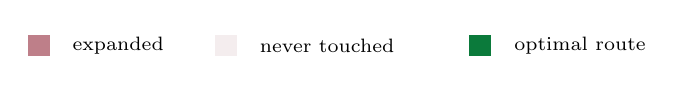
\begin{tikzpicture}[x=0.34cm,y=0.34cm, baseline=0pt]
    \renewcommand{\gpad}{0.09}%
    \gcell{gclose}{0}{0}
      \node[anchor=west, font=\scriptsize] at (1.4,0.5) {expanded};
    \gcell{gfree}{7}{0}
      \node[anchor=west, font=\scriptsize] at (8.4,0.5) {never touched};
    \gcell{cbGreen}{16.5}{0}
      \node[anchor=west, font=\scriptsize] at (17.9,0.5) {optimal route};
  \end{tikzpicture}}

% 3D-e: cone / pyramid, rim at distance 4, sample point P = (2,1)
\def\kE{0.8}\def\pEx{2}\def\pEy{1}


% colour-coded highlight, shown from overlay 2 on: #1 = 2 orange, 3 green,
% 4 blue, 5 red, anything else yellow.  preamble2.tex calls it \hlon; it
% is renamed so it can sit beside part 1's \hlon{<overlay>}{...} in
% combined.tex.
\newcommand{\hlonc}[2]{%
  \alt<2->{%
    \setlength{\fboxsep}{1.4pt}%
    \ifnum#1=2 \colorbox{cbOrange!30}{#2}%
    \else\ifnum#1=3 \colorbox{cbGreen!30}{#2}%
    \else\ifnum#1=4 \colorbox{rblue!30}{#2}%
    \else\ifnum#1=5 \colorbox{cbRed!30}{#2}%
    \else \colorbox{hlyellow}{#2}%
    \fi\fi\fi\fi
  }{#2}%
}

% \subimport: part 3's own \input{visuals}, \input{generated/...}
% resolve relative to its folder
\subimport{part3/}{part3-defs}


\newfontfamily\diagfontsc{lmroman10-}[Extension=.otf,
  UprightFont=*regular, BoldFont=*bold,
  ItalicFont=*italic,   BoldItalicFont=*bolditalic,
  SmallCapsFont=lmromancaps10-regular]
\newcommand{\partsetup}[1]{%
  \ifnum#1=3 \let\algfont\diagfontsc \else \let\algfont\diagfont \fi
  \ifcase#1\or
    \renewcommand{\footauthor}{Zarif Ishmam}%
    \tikzset{sball/.style = {circle, fill=gstart, draw=white, line width=0.7pt,
                             minimum size=3.2mm, inner sep=0pt}}%
    \pgfplotsset{tilesurf/.style = {surf, shader=faceted, faceted color=white,
                                    line width=0.4pt, z buffer=sort, point meta=z}}%
  \or
    \renewcommand{\footauthor}{Proteek Rosul}%
    \tikzset{sball/.style = {circle, fill=gstart, draw=white, line width=0.7pt,
                             minimum size=3.4mm, inner sep=0pt}}%
    \pgfplotsset{tilesurf/.style = {surf, shader=faceted, faceted color=white,
                                    line width=0.45pt, z buffer=sort, point meta=z}}%
  \or
    \renewcommand{\footauthor}{Tonmoy Biswas}%
  \fi}

% ---------- the roadmap banner ------------------------------------------
\newcommand{\parttitle}[1]{\ifcase#1\or Introduction to Pathfinding and A*%
  \or Complexity Analysis and Heuristics\or Worked Simulation\fi}
\newcommand{\partwho}[1]{\ifcase#1\or Zarif Ishmam \,$\cdot$\, 2305035%
  \or Proteek Rosul \,$\cdot$\, 2305042\or Tonmoy Biswas \,$\cdot$\, 2305038\fi}
% three cards, one per part: card #1 is lit, the others muted.  The rail on
% the left marks progress -- parts already given pale, the current one solid.
\newcommand{\partbanner}[1]{%
  \begin{tikzpicture}[
      card/.style    = {rounded corners=3pt, minimum width=11cm,
                        minimum height=1.3cm, inner sep=0pt},
      cardon/.style  = {card, fill=rblue, draw=rbluedk, line width=0.8pt, blkshadow},
      cardoff/.style = {card, fill=rbluelt!60, draw=rbluelt, line width=0.6pt},
      num/.style     = {circle, minimum size=0.78cm, inner sep=0pt,
                        font=\large\bfseries},
      rail/.style    = {circle, minimum size=2.6mm, inner sep=0pt}]
    \draw[rbluelt, line width=1.4pt] (-6.1,0) -- (-6.1,-3.3);
    \foreach \k in {1,2,3}{%
      \pgfmathsetmacro\yy{-1.65*(\k-1)}%
      \ifnum\k=#1
        \node[cardon] (c) at (0,\yy) {};
        \node[num, fill=white, text=rblue] at ($(c.west)+(0.75,0)$) {\k};
        \node[anchor=west, text=white, font=\large\bfseries]
          at ($(c.west)+(1.45,0.2)$) {\parttitle{\k}};
        \node[anchor=west, text=rbluelt, font=\small]
          at ($(c.west)+(1.45,-0.3)$) {\partwho{\k}};
        \node[rail, fill=rblue, draw=white, line width=0.8pt,
              minimum size=3.6mm] at (-6.1,\yy) {};
      \else
        \node[cardoff] (c) at (0,\yy) {};
        \node[num, fill=white, draw=rbluelt, text=gray!55]
          at ($(c.west)+(0.75,0)$) {\k};
        \node[anchor=west, text=gray!60, font=\large]
          at ($(c.west)+(1.45,0.2)$) {\parttitle{\k}};
        \node[anchor=west, text=gray!50, font=\small]
          at ($(c.west)+(1.45,-0.3)$) {\partwho{\k}};
        \ifnum\k<#1
          \node[rail, fill=rbluemd!55] at (-6.1,\yy) {};
        \else
          \node[rail, fill=white, draw=rbluelt, line width=0.8pt] at (-6.1,\yy) {};
        \fi
      \fi}
  \end{tikzpicture}}

\begin{document}

% ---- title
\partsetup{1}
% title.tex -- the deck's title frame (from part 1).  part1_v2_backup.tex
%   shows it when built alone; combined.tex shows it before banner 1
% ---------- 1. TITLE --------------------------------------------------
\begin{frame}[plain]
  \begin{beamercolorbox}[wd=\textwidth,sep=13pt,rounded=true,shadow=true]{title}
    \centering
    {\LARGE\bfseries A* Search Algorithm}\\[7pt]
  \end{beamercolorbox}

  \vspace{2.2em}
  \begin{center}
    \begin{columns}[c]
      \column{0.25\textwidth}
      \begin{center}
        {\large Zarif Ishmam }\\[7pt]
        {\large 2305035}\\[7pt]
      \end{center}
      \vspace{-0.5em}
      \column{0.25\textwidth}
      \begin{center}
        {\large Tonmoy Biswas}\\[7pt]
        {\large 2305038}\\[7pt]
      \end{center}
      \column{0.25\textwidth}
      \begin{center}
        {\large Proteek Rosul}\\[7pt]
        {\large 2305042}
      \end{center}
    \end{columns}
  \end{center}

  \vspace{1.8em}
  \begin{center}
    {\footnotesize\scshape CSE200 $\cdot$ CSE, BUET}
  \end{center}
\end{frame}
               

% ---------- part 1
\begin{frame}{Roadmap}\centering\partbanner{1}\end{frame}
% !TEX program = xelatex
% ======================================================================
%  part1_v2.tex -- A* Search Algorithm, Part 1 (v2)
%      latexmk -xelatex part1_v2.tex
%
%  Assembled from: part1's title frame and applications frame
%  (sec-a-intro.tex), every frame of bd_map.tex, and part1's frame 20
%  (sec-d-limits.tex) re-used as the summary.  Those pieces are copied
%  VERBATIM -- edits to the originals do not flow here, and vice versa.
% ======================================================================
\documentclass[aspectratio=169,10pt]{beamer}

% ======================================================================
%  preamble.tex -- shared by part1.tex, part2.tex, part3.tex
%  A* Search Algorithm -- CSE200, CSE BUET
%  ENGINE: XeLaTeX only (fontspec + OpenType)
% ======================================================================

\usetheme{default}
\useinnertheme{rounded}
\setbeamertemplate{navigation symbols}{}
\setbeamercovered{invisible}

% ----------------------------------------------------------------------
%  1.  FONTS
%      text  -> beamer default  (Latin Modern Sans, beamer's own face)
%      diag  -> Latin Modern Roman  (the LaTeX default face)
%      alg   -> Latin Modern Roman  (the LaTeX default face)
%      math  -> beamer default, untouched
%
%      >>> IBM PLEX SANS: to bring it back as the text font, uncomment
%      >>> the two \set...font lines below.  (TeX Live `plex' fonts,
%      >>> found via kpathsea -- nothing has to live in fonts/.)
% ----------------------------------------------------------------------
\usepackage{fontspec}
% \setmainfont{IBMPlexSans}[Extension=.otf,
%   UprightFont=*-Regular, BoldFont=*-Bold,
%   ItalicFont=*-Italic,   BoldItalicFont=*-BoldItalic]
% \setsansfont{IBMPlexSans}[Extension=.otf,
%   UprightFont=*-Regular, BoldFont=*-Bold,
%   ItalicFont=*-Italic,   BoldItalicFont=*-BoldItalic]
\newfontfamily\diagfont{lmroman10-}[Extension=.otf,
  UprightFont=*regular, BoldFont=*bold,
  ItalicFont=*italic,   BoldItalicFont=*bolditalic]
\let\algfont\diagfont

\usepackage{amsmath,amssymb,mathtools}
\usepackage{booktabs}
\usepackage{pifont}                % \ding symbols (part 2)
\usepackage[table]{xcolor}
\usepackage{graphicx}
\usepackage{tikz}
\usetikzlibrary{arrows.meta,positioning,decorations.pathreplacing,calc,
                shapes.geometric,backgrounds,fit,shadows.blur, tikzmark}

% ----------------------------------------------------------------------
%  2.  PALETTE
% ----------------------------------------------------------------------
\definecolor{rblue}{HTML}{2E2E9C}
\definecolor{rbluedk}{HTML}{1C1C6B}
\definecolor{rbluemd}{HTML}{5A5AC4}
\definecolor{rbluelt}{HTML}{E7E7F7}
\definecolor{cbOrange}{HTML}{D97706}
\definecolor{cbOrangeLt}{HTML}{FDF0DC}
\definecolor{cbGreen}{HTML}{0B7A3B}
\definecolor{cbGreenLt}{HTML}{E4F2E9}
\definecolor{cbRed}{HTML}{B01B2E}
\definecolor{cbRedLt}{HTML}{FAE7E9}
\definecolor{crison}{HTML}{96383c}
\definecolor{neutralg}{gray}{0.46}
\definecolor{lnnum}{gray}{0.58}
\definecolor{hlyellow}{HTML}{FFE9A8}
\definecolor{gridgray}{gray}{0.82}
\definecolor{closedc}{gray}{0.80}

% grid tiles -- flat, low-saturation rose ramp: untouched -> frontier ->
% expanded, plus a charcoal wall.  S and G are solid accent tiles.
\definecolor{gfree}{HTML}{F4EDEE}
\definecolor{gopen}{HTML}{DEBBC2}
\definecolor{gclose}{HTML}{BE7F89}
\definecolor{gwall}{HTML}{3F3F46}
\definecolor{gstart}{HTML}{0B7A3B}
\definecolor{ggoal}{HTML}{B01B2E}

% soft, low-saturation tints used only by the beamer blocks -- kept apart
% from the tikz palette above so diagram colours stay untouched
\definecolor{blkInk}{HTML}{20242E}
\definecolor{blkBlueTt}{HTML}{E4E4F3}
\definecolor{blkBlueBd}{HTML}{F3F3FA}
\definecolor{blkBlueFg}{HTML}{2E2E78}
\definecolor{blkRedTt}{HTML}{F4E4E6}
\definecolor{blkRedBd}{HTML}{FBF4F4}
\definecolor{blkRedFg}{HTML}{8C2C3A}
\definecolor{blkGrnTt}{HTML}{E2EEE7}
\definecolor{blkGrnBd}{HTML}{F2F8F4}
\definecolor{blkGrnFg}{HTML}{2E6A4A}

\newcommand{\pos}[1]{\textcolor{cbGreen}{#1}}
\newcommand{\con}[1]{\textcolor{cbOrange}{#1}}
\newcommand{\bad}[1]{\textcolor{cbRed}{#1}}
\newcommand{\HL}[1]{\textcolor{rblue}{#1}}
\newcommand{\mut}[1]{\textcolor{neutralg}{#1}}

% ----------------------------------------------------------------------
%  3.  COLOUR ASSIGNMENTS
% ----------------------------------------------------------------------
\setbeamercolor{structure}{fg=rblue}
\setbeamercolor{frametitle}{bg=rblue,fg=white}
\setbeamercolor{title}{bg=rblue,fg=white}
\setbeamercolor{block title}{bg=blkBlueTt,fg=blkBlueFg}
\setbeamercolor{block body}{bg=blkBlueBd,fg=blkInk}
\setbeamercolor{block title alerted}{bg=blkRedTt,fg=blkRedFg}
\setbeamercolor{block body alerted}{bg=blkRedBd,fg=blkInk}
\setbeamercolor{block title example}{bg=blkGrnTt,fg=blkGrnFg}
\setbeamercolor{block body example}{bg=blkGrnBd,fg=blkInk}
\setbeamercolor{itemize item}{fg=rblue}
\setbeamercolor{itemize subitem}{fg=rbluemd}
\setbeamercolor{alerted text}{fg=cbRed}

\setbeamertemplate{blocks}[default]

% Square corners WITH a shadow.  Beamer offers shadow= only on the
% [rounded] variant, so the shadow is added by hand here: each block is
% captured into \blkbox, then dropped into a tikz node that carries the
% shadow.  Geometry stays beamer's [default] block, i.e. square.
%
%      >>> NO SHADOW: comment out the six \setbeamertemplate lines at the
%      >>> end of this block; [default] above then takes over again.
\usetikzlibrary{shadows}
\newsavebox{\blkbox}
\tikzset{blkshadow/.style={drop shadow={shadow xshift=1.3pt,
                                        shadow yshift=-1.3pt,
                                        opacity=0.20, fill=black!70}}}

\newcommand{\blkopen}[2]{%   #1 = title beamercolor, #2 = body beamercolor
  \par\vskip\medskipamount%
  \begin{lrbox}{\blkbox}%
  \begin{minipage}{\textwidth}%
    \begin{beamercolorbox}[colsep*=.75ex]{#1}%
      \usebeamerfont*{block title}\insertblocktitle%
    \end{beamercolorbox}%
    {\parskip0pt\par}%
    \nointerlineskip%
    \usebeamerfont{block body}%
    \begin{beamercolorbox}[colsep*=.75ex,vmode]{#2}%
      \vskip-.75ex\vbox{}%
}
\newcommand{\blkclose}{%
    \end{beamercolorbox}%
  \end{minipage}%
  \end{lrbox}%
  % The picture is 1.5ex wider than \textwidth (see inner xsep below), so
  % it is parked in a \textwidth hbox with \hss to absorb the overhang --
  % otherwise every block reports an Overfull \hbox.  The -.75ex shift
  % puts the bleed on both sides, exactly where stock beamer puts it.
  \noindent\hbox to\textwidth{\hspace*{-.75ex}%
  \begin{tikzpicture}
    % inner xsep matches the .75ex that colsep* bleeds outside the box,
    % so the node path (and therefore the shadow) covers the painted block
    \node[inner xsep=.75ex, inner ysep=0pt, outer sep=0pt, blkshadow]
          {\usebox{\blkbox}};
  \end{tikzpicture}\hss}%
  \vskip\smallskipamount%
}

\setbeamertemplate{block begin}{\blkopen{block title}{block body}}
\setbeamertemplate{block end}{\blkclose}
\setbeamertemplate{block alerted begin}{\blkopen{block title alerted}{block body alerted}}
\setbeamertemplate{block alerted end}{\blkclose}
\setbeamertemplate{block example begin}{\blkopen{block title example}{block body example}}
\setbeamertemplate{block example end}{\blkclose}

% for triangle and square
% \setbeamertemplate{itemize item}{\raisebox{0.1ex}{\scriptsize$\blacktriangleright$}}
% \setbeamertemplate{itemize subitem}{\raisebox{0.1ex}{\tiny$\blacksquare$}}
% for circle and square
\setbeamertemplate{itemize item}{\raisebox{0.1ex}{\scriptsize$\bullet$}}
\setbeamertemplate{itemize subitem}{\raisebox{0.1ex}{\tiny$\blacksquare$}}

\setbeamerfont{frametitle}{size=\large,series=\bfseries}
\setbeamerfont{block title}{size=\small,series=\bfseries}
\setbeamerfont{footline}{size=\scriptsize}
\setbeamerfont{footnote}{size=\tiny}
% beamer's default footnote template indents by \parindent 1em and puts the
% marker in a 1.8em box; both are dropped here so the note sits flush left
\setbeamertemplate{footnote}{%
  \parindent0em\noindent\raggedright
  \usebeamerfont{footnote}%
  \hbox to 0.9em{\insertfootnotemark\hfil}\insertfootnotetext\par}

% ----------------------------------------------------------------------
%  4.  FRAME TITLE
% ----------------------------------------------------------------------
\setbeamertemplate{frametitle}{%
  \nointerlineskip
  \begin{beamercolorbox}[wd=\paperwidth,ht=3.4ex,dp=1.5ex,%
                         leftskip=1.6ex,rightskip=1.6ex]{frametitle}
    \usebeamerfont{frametitle}\insertframetitle
  \end{beamercolorbox}%
}

% ----------------------------------------------------------------------
%  4b. CORNER MOTIF  (faint search lattice, right end of the title bar)
%      A 4x3 grid graph with the staircase route traced from a filled
%      start node to a double-ringed goal -- the picture A* is about.
%      Tints are mixed against rblue so it reads as a watermark on the
%      bar.  It lives INSIDE the title bar because the longest frame
%      title stops at 12.6cm of 16cm, so that strip is always free --
%      anywhere in the body area it would clash with wide text lines.
%
%      >>> TO TURN IT OFF: comment out the \addtobeamertemplate line at
%      >>> the bottom of this block (put a % in front of it). Leave
%      >>> \cornermotif defined; nothing else refers to it.
% ----------------------------------------------------------------------
\newcommand{\motifstep}{0.30cm}      % lattice pitch
\newcommand{\cornermotif}{%
  \begin{tikzpicture}[remember picture, overlay,
      mn/.style    = {circle, draw=white!38!rblue, line width=0.4pt,
                      fill=white!20!rblue, minimum size=1.5mm, inner sep=0pt},
      mon/.style   = {mn, draw=white!62!rblue, fill=white!44!rblue},
      me/.style    = {draw=white!30!rblue, line width=0.4pt},
      mpath/.style = {draw=white!68!rblue, line width=0.8pt,
                      line cap=round, line join=round}]
    \begin{scope}[shift={($(current page.north east)+(-1.45cm,-0.88cm)$)},
                  x=\motifstep, y=\motifstep]
      \foreach \c in {0,1,2,3}{\draw[me] (\c,0) -- (\c,2);}
      \foreach \r in {0,1,2}  {\draw[me] (0,\r) -- (3,\r);}
      \draw[mpath] (0,0) -- (1,0) -- (1,1) -- (2,1) -- (2,2) -- (3,2);
      \foreach \c in {0,1,2,3}{\foreach \r in {0,1,2}{\node[mn] at (\c,\r) {};}}
      \foreach \q in {(1,0),(1,1),(2,1),(2,2)}{\node[mon] at \q {};}
      \node[mn, fill=white!88!rblue, draw=white!88!rblue] at (0,0) {};
      \node[mn, draw=white!88!rblue, double, double distance=0.35pt] at (3,2) {};
    \end{scope}
  \end{tikzpicture}%
}
\addtobeamertemplate{frametitle}{}{\cornermotif}

% ----------------------------------------------------------------------
%  GLOBAL VERTICAL NUDGE
%  One knob for the whole deck: space added just under the title bar, so
%  every titled frame's content sits lower.  The frame body is centred, so
%  the visible shift is HALF of this value.  The [plain] title slide has no
%  frametitle and is untouched.  Set to 0pt to disable.
% ----------------------------------------------------------------------
\newlength{\framenudge}
\setlength{\framenudge}{4pt}
\addtobeamertemplate{frametitle}{}{\vskip\framenudge}


% ----------------------------------------------------------------------
%  5.  FOOTER
%        ----------------------------------------------------------
%        CSE200 - A* Search Algorithm   Zarif Ishmam      n / N
%      ============                                    <- progress
% ----------------------------------------------------------------------
\newcommand{\footcourse}{CSE200 - A* Search Algorithm}
\newcommand{\footauthor}{Zarif Ishmam}
\newcommand{\pbheight}{1.5pt}

\newcommand{\progressbarline}{%
  \ifnum\inserttotalframenumber>0\relax
    % capped at 1: on a first pass the total is not known yet, and in a
    % long deck n/total would make the bar wider than TeX can measure
    \pgfmathsetmacro{\pbfrac}{min(1,\insertframenumber/\inserttotalframenumber)}%
  \else
    \def\pbfrac{0}%
  \fi
  \noindent
  \textcolor{rblue}{\rule{\pbfrac\paperwidth}{\pbheight}}%
  \textcolor{rblue!14}{\rule{\dimexpr\paperwidth-\pbfrac\paperwidth\relax}{\pbheight}}%
}

\setbeamercolor{footbar}{bg=white,fg=rbluedk}
\newcommand{\footmargin}{1.8ex}
\setbeamertemplate{footline}{%
  \noindent\hspace*{\footmargin}%
  \textcolor{gray!45}{%
    \rule{\dimexpr\paperwidth-\footmargin-\footmargin\relax}{0.4pt}}%
  \hspace*{\footmargin}%
  \vskip1.5pt
  \hbox{%
    \begin{beamercolorbox}[wd=\paperwidth,ht=2.1ex,dp=0.8ex,%
                           leftskip=\footmargin,rightskip=\footmargin]{footbar}%
      \usebeamerfont{footline}\diagfont
      % zero-width boxes: the two \hfill split the strip evenly, so the
      % author sits on the exact centre line regardless of the side widths
      \makebox[0pt][l]{\textsc{\footcourse}}%
      \hfill
      \makebox[0pt][c]{\textsc{\footauthor}}%
      \hfill
      \makebox[0pt][r]{\textsc{\insertframenumber\,/\,\inserttotalframenumber}}%
    \end{beamercolorbox}%
  }%
  \vskip1pt%
  \progressbarline
  \vskip0pt%
}

% ----------------------------------------------------------------------
%  6.  CLRS-STYLE ALGORITHM  (default LaTeX face, line numbered, overlay aware)
% ----------------------------------------------------------------------
\newcounter{alglin}
\newcommand{\kw}[1]{\textcolor{rblue}{\textbf{#1}}}
\newcommand{\proc}[1]{\textsc{#1}}
\newcommand{\com}[1]{\textcolor{neutralg}{\itshape\,\(\triangleright\) #1}}
\newcommand{\idt}[1]{\hspace*{#1\dimexpr1.25em\relax}}
\newcommand{\hlon}[2]{\alt<#1>{\setlength{\fboxsep}{1.4pt}\colorbox{hlyellow}{#2}}{#2}}

% Stacked hboxes, not a tabular: LaTeX puts \@arstrut in every tabular row,
% so a hidden line still claimed a full line of height and the block never
% shrank.  As plain hboxes a hidden \aline contributes nothing at all, which
% lets the frame centre on the lines actually showing.
\newenvironment{clrs}[1][\small]
  {\begingroup\algfont#1\setcounter{alglin}{0}%
   \setlength{\parindent}{0pt}\setlength{\parskip}{0pt}%
   \begin{minipage}[t]{\linewidth}}
  {\end{minipage}\endgroup}

\newcommand{\aline}[2][1-]{%
  \stepcounter{alglin}%
  \only<#1>{\hbox{\hbox to 1.15em{\hfil\textcolor{lnnum}{\scriptsize\thealglin}}%
                  \hspace{1.3ex}\strut#2}}}

% ----------------------------------------------------------------------
%  7.  TIKZ STYLES
% ----------------------------------------------------------------------
\tikzset{
  every picture/.append style={font=\diagfont},
  vtx/.style      = {circle, draw=rbluedk, line width=0.7pt, fill=white,
                     minimum size=6.5mm, inner sep=0pt, font=\small},
  vstart/.style   = {vtx, fill=cbGreenLt, draw=cbGreen, line width=1.1pt,
                     font=\small\bfseries},
  vgoal/.style    = {vtx, fill=cbRedLt, draw=cbRed, line width=1.1pt,
                     font=\small\bfseries, double, double distance=0.6pt},
  vopen/.style    = {vtx, fill=rbluelt, draw=rblue, line width=1.1pt},
  vclosed/.style  = {vtx, fill=closedc, draw=neutralg, line width=0.9pt},
  vcur/.style     = {vtx, fill=hlyellow, draw=cbOrange, line width=1.3pt},
  edg/.style      = {draw=neutralg, line width=0.8pt},
  edgon/.style    = {draw=rblue, line width=1.6pt},
  edgpath/.style  = {draw=cbGreen, line width=2.2pt},
  edggrey/.style  = {draw=gridgray, line width=1.6pt},
  edgdead/.style  = {draw=gridgray, line width=0.6pt},
  edgorange/.style= {draw=cbOrange, line width=2.2pt},
  arr/.style      = {-{Stealth[length=2.4mm]}, line width=1.0pt},
  wlab/.style     = {font=\scriptsize, fill=white, inner sep=1pt, text=rbluedk},
  hlab/.style     = {font=\scriptsize, text=cbOrange, inner sep=1pt},
  box/.style      = {draw=rbluedk, rounded corners=2pt, fill=rbluelt,
                     minimum width=2.3cm, minimum height=0.8cm,
                     font=\small, align=center},
  boxg/.style     = {box, fill=cbGreenLt, draw=cbGreen},
  boxr/.style     = {box, fill=cbRedLt,   draw=cbRed},
  boxo/.style     = {box, fill=cbOrangeLt, draw=cbOrange},
}

% ----------------------------------------------------------------------
%  8.  THE SHARED 16 x 10 GRID
%      cell (c,r) spans [c,c+1] x [r,r+1];  centre (c+.5, r+.5)
%      S = (1,4)   G = (14,6)
%      Walls form a U that opens WEST, straight at the start, so a greedy
%      search walks into it.  Verified numbers on this map:
%        Dijkstra 137 cells / cost 19   Greedy 48 / cost 35   A* 81 / cost 19
% ----------------------------------------------------------------------
\newcommand{\gridnodefont}{\tiny\bfseries}
\newcommand{\gridnodeS}{S}
\newcommand{\gridnodeG}{G}

% --- flat-tile look: every cell is its own square, separated by a gutter.
%     No grid rules, no outer frame -- the gutters do all the separating.
\newcommand{\gpad}{0.075}               % gutter half-width, in cell units
\newcommand{\gcell}[3]{%                % #1 = colour, #2 = col, #3 = row
  \fill[#1] ({#2+\gpad},{#3+\gpad}) rectangle ({#2+1-\gpad},{#3+1-\gpad});}
\newcommand{\gletter}[4]{%              % #1 = colour, #2 = col, #3 = row, #4 = glyph
  \gcell{#1}{#2}{#3}%
  \node[text=white, font=\gridnodefont, inner sep=0pt]
        at ({#2+0.5},{#3+0.5}) {#4};}

% the wall set: a U opening WEST
\newcommand{\gwalls}{%
  \foreach \c in {4,...,12} {\gcell{gwall}{\c}{3}\gcell{gwall}{\c}{7}}%
  \foreach \r in {4,5,6} {\gcell{gwall}{12}{\r}}}

% laid down FIRST, under everything the search paints
\newcommand{\gridback}{%
  \foreach \c in {0,...,15} {\foreach \r in {0,...,9} {\gcell{gfree}{\c}{\r}}}}

% laid down LAST, over everything the search paints
\newcommand{\drawgridbase}{%
  \gwalls
  \gletter{gstart}{1}{4}{\gridnodeS}%
  \gletter{ggoal}{14}{6}{\gridnodeG}%
}

% full-size grid picture; #1 = cell size, #2 = generated body file
\newcommand{\gridpic}[2]{%
  \begin{tikzpicture}[x=#1, y=#1]
    \gridback
    \input{#2}
  \end{tikzpicture}}

% reduced grid picture for side-by-side panels
\newcommand{\gridpicsmall}[2]{%
  \begingroup
    \renewcommand{\gridnodefont}{\fontsize{3.6}{4}\selectfont\bfseries}%
    \begin{tikzpicture}[x=#1, y=#1]
      \gridback
      \input{#2}
    \end{tikzpicture}%
  \endgroup}

% tiny panels: tiles only, no letters
\newcommand{\gridpictiny}[2]{%
  \begingroup
    \renewcommand{\gpad}{0.10}%
    \renewcommand{\gridnodeS}{}\renewcommand{\gridnodeG}{}%
    \begin{tikzpicture}[x=#1, y=#1]
      \gridback
      \input{#2}
    \end{tikzpicture}%
  \endgroup}

% legend strip used under the grid frames
\newcommand{\gridlegend}{%
  
\begin{tikzpicture}[x=0.34cm,y=0.34cm, baseline=0pt]
    \renewcommand{\gpad}{0.09}%
    \gcell{gclose}{0}{0}
      \node[anchor=west, font=\tiny] at (1.4,0.5) {closed};
    \gcell{gopen}{5.4}{0}
      \node[anchor=west, font=\tiny] at (6.8,0.5) {open (frontier)};
    \gcell{cbGreen}{15.0}{0}
      \node[anchor=west, font=\tiny] at (16.4,0.5) {final path};
    \gcell{gwall}{21.4}{0}
      \node[anchor=west, font=\tiny] at (22.8,0.5) {wall};
  \end{tikzpicture}}

% grey until overlay #1, bold blue on it, dark from then on
\newcommand{\lit}[2]{%
  \temporal<#1>{\textcolor{gray!50}{#2}}%
               {\textcolor{rblue}{\textbf{#2}}}%
               {\textcolor{rbluedk}{#2}}}

\newcommand{\takeaway}[1]{%
  \vfill
  \begin{beamercolorbox}[wd=\textwidth,sep=4pt,rounded=true]{block body}
    \footnotesize\textbf{Takeaway.} #1
  \end{beamercolorbox}}

\newcommand{\statdijkstraexp}{137}
\newcommand{\statdijkstrapath}{19}
\newcommand{\statgreedyexp}{48}
\newcommand{\statgreedypath}{35}
\newcommand{\statastarexp}{81}
\newcommand{\statastarpath}{19}

\input{part1-defs}          % part 1 macros (also loaded by combined.tex)
\begin{document}

% static artwork, drawn once for the whole deck (see the SPEED notes)
\bdmakebox
\sbox{\gpdj}{\gridpanel{dj}{\dijkstraroute}{cbGreen}}
\sbox{\gpgr}{\gridpanel{gr}{\greedyroute}{cbOrange}}
\sbox{\gpas}{\gridpanel{as}{\astarroute}{cbGreen}}

% the title frame lives in title.tex: combined.tex shows it before the
% roadmap banner, so a combined build skips it here
\ifdefined\combineddeck\else% title.tex -- the deck's title frame (from part 1).  part1_v2_backup.tex
%   shows it when built alone; combined.tex shows it before banner 1
% ---------- 1. TITLE --------------------------------------------------
\begin{frame}[plain]
  \begin{beamercolorbox}[wd=\textwidth,sep=13pt,rounded=true,shadow=true]{title}
    \centering
    {\LARGE\bfseries A* Search Algorithm}\\[7pt]
  \end{beamercolorbox}

  \vspace{2.2em}
  \begin{center}
    \begin{columns}[c]
      \column{0.25\textwidth}
      \begin{center}
        {\large Zarif Ishmam }\\[7pt]
        {\large 2305035}\\[7pt]
      \end{center}
      \vspace{-0.5em}
      \column{0.25\textwidth}
      \begin{center}
        {\large Tonmoy Biswas}\\[7pt]
        {\large 2305038}\\[7pt]
      \end{center}
      \column{0.25\textwidth}
      \begin{center}
        {\large Proteek Rosul}\\[7pt]
        {\large 2305042}
      \end{center}
    \end{columns}
  \end{center}

  \vspace{1.8em}
  \begin{center}
    {\footnotesize\scshape CSE200 $\cdot$ CSE, BUET}
  \end{center}
\end{frame}
\fi

% ---------- PATHFINDING -----------------------------------------------
\begin{frame}{Pathfinding}
  \vspace{-2em}
  \begin{block}{Pathfinding}
    The problem of simply finding a \textbf{valid path} from any point
    \textcolor{cbGreen}{\textbf{A}} to any point \textcolor{cbRed}{\textbf{B}}
    in a graph.
  \end{block}

  \vspace{3em}
  \begin{columns}[c]
    \column{0.44\textwidth} 

      \centering
      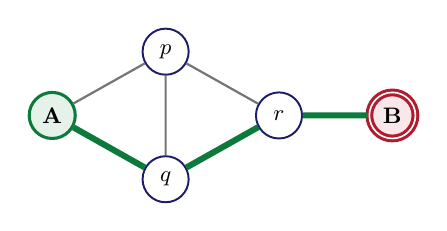
\begin{tikzpicture}[scale=0.9, transform shape]
        \node[vstart] (A) at (0,0.9)   {A};
        \node[vtx]    (p) at (1.6,1.8) {$p$};
        \node[vtx]    (q) at (1.6,0)   {$q$};
        \node[vtx]    (r) at (3.2,0.9) {$r$};
        \node[vgoal]  (B) at (4.8,0.9) {B};
        \draw[edg] (A)--(p) (A)--(q) (p)--(q) (p)--(r) (q)--(r) (r)--(B);
        \only<2->{\draw[edgpath] (A)--(q)--(r)--(B);}
      \end{tikzpicture}\par\vspace{4pt}

    \column{0.52\textwidth}
      \centering
      \begingroup
        \renewcommand{\gridnodeS}{A}\renewcommand{\gridnodeG}{B}%
        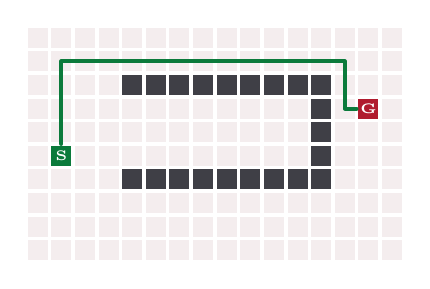
\begin{tikzpicture}[x=0.30cm, y=0.30cm]
          \gridback
          \drawgridbase
          \only<2->{\draw[cbGreen, line width=1.4pt, line cap=round,
                          line join=round]
            (1.5,5) -- (1.5,8.5) -- (13.5,8.5) -- (13.5,6.5) -- (14,6.5);}
        \end{tikzpicture}\par\vspace{4pt}
      \endgroup
  \end{columns}
\end{frame}

% ---------- 9. APPLICATIONS -------------------------------------------
% \urldef grabs these at top level: inside \footnote{...} the # and _ in the
% wikipedia link would be tokenised before \url could make them harmless.
\urldef{\urlpathfinding}\url{https://www.nature.com/articles/s41467-026-75254-8}
\urldef{\urlproteinfold}\url{https://en.wikipedia.org/wiki/Protein_folding#/media/File:ACBP_MSM_from_Folding@home.tiff}

\begin{frame}{Where pathfinding is used}
  \begin{columns}[T]
    \column{0.46\textwidth}
      \begin{center}
        \only<1-2>{%
          \includegraphics[width=5.6cm,height=4.1cm,keepaspectratio]%
            {images/app-pathfinding.png}%
          \footnote[frame]{Image source: \urlpathfinding}}
        \only<3>{%
          % photo, replaced by the 3D game map below -- to bring it back,
          % uncomment these two lines and comment out \gamemap ... \gamelegend
          % \includegraphics[width=5.6cm,height=4.1cm,keepaspectratio]%
          %   {images/app-game.png}%
          \gamemap\par\vspace{3pt}
          \gamelegend
          }
        \only<4>{%
          \includegraphics[width=5.6cm,height=4.1cm,keepaspectratio]%
            {images/app-networking.png}%
        }
        \only<5>{%
          \includegraphics[width=5.6cm,height=4.1cm,keepaspectratio]%
            {images/app-proteinfolding.png}%
          \footnote[frame]{Image source: \urlproteinfold}}
        \only<6>{%
          \includegraphics[width=5.6cm,height=4.1cm,keepaspectratio]%
            {images/app-more.png}%
        }
      \end{center}

    \column{0.50\textwidth}
      \begin{itemize}\setlength{\itemsep}{11pt}
        \item \lit{2}{Road navigation}\\
        \item \lit{3}{Game AI and NPC movement}\\
        \item \lit{4}{Networks and packet routing}\\
        \item \lit{5}{Protein folding}\\
        \item \lit{6}{\ldots{}and many more}\\
              {\scriptsize\mut{Puzzles, Robotics, Dependency resolution}}
      \end{itemize}
  \end{columns}
\end{frame}

% ---------- TWO REQUIREMENTS ------------------------------------------
\begin{frame}{Two requirements}
  \begin{center}
  
\begin{tikzpicture}
    \node<1->[draw=rblue, fill=rbluelt, rounded corners=3pt, line width=1pt,
        text width=4.8cm, align=center, inner sep=12pt] at (0,0)
      {{\small\mut{1}}\\[3pt]{\bfseries\large\HL{Shortest path}}};
    \node<1->[draw=cbOrange, fill=cbOrangeLt, rounded corners=3pt,
        line width=1pt, text width=4.8cm, align=center, inner sep=12pt]
        at (6.2,0)
      {{\small\mut{2}}\\[3pt]{\bfseries\large\con{Efficient algorithm}}};
  \end{tikzpicture}
  \end{center}
\end{frame}

% ---------- A REAL GRAPH: BANGLADESH ----------------------------------
\begin{frame}{A real graph --- the 64 districts of Bangladesh}
  \centering
  \begin{tikzpicture}[x=\bdscalex, y=\bdscaley,
                      shift={(-87.98,-20.75)}, every node/.style={inner sep=0pt}]
    \bdbase \bdends \bdlabels
  \end{tikzpicture}
  \par\vspace{0.4em}
  {\small Let's look at an example of a path from
   \textcolor{cbGreen}{\textbf{Dhaka}} to \textcolor{cbGreen}{\textbf{Sylhet}}.}
\end{frame}

% ================= from bd_map.tex (all frames, verbatim) ============
% ======================================================================
%  1.  THE ALGORITHM, THEN WHAT IT MEANS
%      ov1  whole pseudocode, unhighlighted, nothing on the right
%      ov2  the block frame appears
%      ov3-5  one bullet at a time, each spotlighting its own lines
% ======================================================================
\begin{frame}[t]{Shortest Path --- Dijkstra's Algorithm}
  \begin{columns}[T]

    \column{0.5\textwidth}
    \begin{clrs}[\footnotesize]
      \aline[1-]{\proc{Dijkstra}$(G, s, t)$}
      \aline[1-]{\idt1 \kw{for each} $v \in V$: \
        $g[v] \gets \infty$,\; $\pi[v] \gets \textsc{nil}$}
      \aline[1-]{\idt1 $g[s] \gets 0$}
      \aline[1-]{\idt1 \hlon{3}{$Q \gets$
        priority queue keyed by $g$, holding $\{s\}$}}
      \aline[1-]{\idt1 $\mathit{S} \gets \varnothing$}
      \aline[1-]{\idt1 \hlon{4}{\kw{while} $Q \neq \varnothing$}}
      \aline[1-]{\idt2 \hlon{4}{$u \gets
        \textsc{Extract-Min}(Q)$}}
      \aline[1-]{\idt2 \kw{if} $u = t$:}
      \aline[1-]{\idt3 \kw{return} \proc{Reconstruct}$(\pi, t)$}
      \aline[1-]{\idt2 \hlon{4}{$\mathit{S} \gets \mathit{S} \cup \{u\}$}}
      \aline[1-]{\idt2 \hlon{5}{\kw{for each} $v$
        adjacent to $u$}}
      \aline[1-]{\idt3 \hlon{5}{\kw{if} $v \in \mathit{S}$: \ \kw{continue}}}
      \aline[1-]{\idt3 \hlon{5}{\kw{if} $g[u] + w(u,v) < g[v]$}}
      \aline[1-]{\idt4 \hlon{5}{$g[v] \gets g[u] + w(u,v)$,\;
        $\pi[v] \gets u$}}
      \aline[1-]{\idt4 \hlon{5}{\textsc{Insert-or-Decrease-Key}
        $(Q, v, g[v])$}}
    \end{clrs}

    \column{0.5\textwidth}
    \onslide<2->{%
    \begin{block}{How Dijkstra picks}
      \small
      \begin{itemize}\setlength{\itemsep}{6pt}
        \item<3-> Start from the source 
        \item<4-> In each iteration, Picks the \textbf{locally best} node so far
        \item<5-> Explores paths for that node
      \end{itemize}
    \end{block}}

  \end{columns}
\end{frame}

% one line of a step list (the three map frames): grey, except on its
% own overlay #1, where it turns bold in colour #2 behind a marker
\newcommand{\stepline}[3]{% #1 overlay, #2 colour, #3 text
  \noindent\alt<#1>{\textcolor{#2}{\makebox[1.1em][l]{\tiny$\blacktriangleright$}\textbf{#3}}}%
                   {\textcolor{gray!50}{\makebox[1.1em][l]{}#3}}\par}

% ======================================================================
%  2.  THE SAME THREE RULES, RUN ON THE MAP
%      ov1    map + the block carried over from frame 1
%      ov2-6  iterations 1..5, the settled set growing outward
%      ov7    right column cleared; the answer as a flow chart
% ======================================================================
\begin{frame}{Dhaka to Sylhet (using Dijkstra's algorithm)}
  \begin{columns}[T]
  \column{0.50\textwidth}
    \centering
    \begin{tikzpicture}[x=\bdscalex, y=\bdscaley,
                        shift={(-87.98,-20.75)}, every node/.style={inner sep=0pt}]
      \bdbase
    \bdtreeedges{2}{dhaka/gazipur, dhaka/narayanganj, dhaka/munshiganj, dhaka/narsingdi,
                     dhaka/manikganj, munshiganj/chandpur, narsingdi/brahmanbaria, munshiganj/shariatpur,
                     manikganj/faridpur, gazipur/tangail}
    \bdtreeedges{3}{manikganj/rajbari, gazipur/kishoreganj, shariatpur/madaripur, munshiganj/cumilla,
                     gazipur/mymensingh, chandpur/lakshmipur, tangail/sirajganj, rajbari/magura,
                     rajbari/pabna, brahmanbaria/habiganj}
    \bdtreeedges{4}{shariatpur/barishal, kishoreganj/netrokona, madaripur/gopalganj, lakshmipur/noakhali,
                     rajbari/kushtia, lakshmipur/bhola, magura/jhenaidah, barishal/jhalokati,
                     cumilla/feni, tangail/jamalpur}
    \bdtreeedges{5}{mymensingh/sherpur, magura/narail, sirajganj/bogura, habiganj/moulvibazar,
                     barishal/patuakhali, gopalganj/bagerhat, barishal/pirojpur, kushtia/chuadanga,
                     sirajganj/natore, narail/jashore}
    \bdtreeedges{6}{kushtia/meherpur, narail/khulna, patuakhali/barguna, netrokona/sunamganj,
                     bogura/joypurhat, bogura/naogaon, feni/khagrachhari, jamalpur/gaibandha,
                     moulvibazar/sylhet}

    \bdring{2}{gazipur, narayanganj, munshiganj, narsingdi, manikganj,
               chandpur, brahmanbaria, shariatpur, faridpur, tangail}
    \bdring{3}{rajbari, kishoreganj, madaripur, cumilla, mymensingh,
               lakshmipur, sirajganj, magura, pabna, habiganj}
    \bdring{4}{barishal, netrokona, gopalganj, noakhali, kushtia,
               bhola, jhenaidah, jhalokati, feni, jamalpur}
    \bdring{5}{sherpur, narail, bogura, moulvibazar, patuakhali,
               bagerhat, pirojpur, chuadanga, natore, jashore}
    \bdring{6}{meherpur, khulna, barguna, sunamganj, joypurhat,
               naogaon, khagrachhari, gaibandha, sylhet}
      \only<7->{\bdroute}
      \bdends
      \bdlabels
      \only<7->{\bdroutelabels}
    \end{tikzpicture}

  \column{0.5\textwidth}
    \only<1-6>{%
      \begin{block}{How Dijkstra picks}
        \small
        \begin{itemize}\setlength{\itemsep}{6pt}
          \item In each step, looks in every direction
          \item Picks the \textbf{locally best} node
          \item Explores paths for that node
        \end{itemize}
      \end{block}
      \vspace{0.9em}
      {\scriptsize\setlength{\parskip}{2pt}%
       \stepline{2}{rblue}{Iteration 1}%
       \stepline{3}{rblue}{Iteration 2}%
       \stepline{4}{rblue}{Iteration 3}%
       \stepline{5}{rblue}{Iteration 4}%
       \stepline{6}{rblue}{Iteration 5}}}%
    \only<7>{%
      \centering
      {\footnotesize\textcolor{cbGreen}{\textbf{Path found}}}\par
      \vspace{0.5em}
      \pathflow}
  \end{columns}
\end{frame}

% ======================================================================
%  3.  WHAT THE SEARCH COST, AND WHAT MAKES DIJKSTRA BAD
%      ov1  map, route and the results table
%      ov2  red arrows to three districts it did not need + bullet 1
%      ov3  bullet 2 -- the greedy heuristic
%      ("What makes Dijkstra bad?" is folded in here; the old frame is
%       kept switched off just below)
% ======================================================================
\begin{frame}{Dhaka to Sylhet --- what the search cost}
  \begin{columns}[c]
  \column{0.50\textwidth}
    \centering
    \begin{tikzpicture}[x=\bdscalex, y=\bdscaley,
                        shift={(-87.98,-20.75)}, every node/.style={inner sep=0pt}]
      \bdbase \bdsettled \bdroute \bdends \bdlabels \bdroutelabels
      \begin{scope}[crimson, line width=0.7pt, opacity=0.9,
                    -{Stealth[length=1.5mm]}]
        \only<2->{\draw (dhaka) to[bend right=14] (jashore);}
        \only<2->{\draw (dhaka) to[bend left=16]  (naogaon);}
        \only<2->{\draw (dhaka) to[bend left=14]  (chattogram);}
      \end{scope}
      \only<2->{\node[bdlab, text=crimson, anchor=south east, xshift=-0.8mm, yshift=0.4mm] at (jashore) {Jashore};}
      \only<2->{\node[bdlab, text=crimson, anchor=east,  xshift=-1.2mm] at (naogaon)    {Naogaon};}
      \only<2->{\node[bdlab, text=crimson, anchor=west,  xshift= 1.2mm] at (chattogram) {Chattogram};}
    \end{tikzpicture}

  \column{0.50\textwidth}
    {\footnotesize
    \begin{tabular}{@{}l@{\hspace{2.2em}}l@{}}
      \toprule
      \textbf{Result} & \\
      \midrule
      Districts on the route & \textbf{6} of 64\\[2pt]
      Districts explored     & \textbf{50} of 64\\[2pt]
      Optimal path?          & \textcolor{cbGreen}{\textbf{Yes}}\\
      \bottomrule
    \end{tabular}\par}
    \vspace{1.4em}
    {\small
    \begin{itemize}\setlength{\itemsep}{12pt}
      \item<2-> Dijkstra explores \textcolor{crimson}{in every direction}.
      \item<3-> We can solve this using a \textcolor{rblue}{\textbf{greedy
            heuristic}}.
    \end{itemize}\par}
  \end{columns}
\end{frame}

% ---------- WHAT MAKES DIJKSTRA BAD? -- switched off ------------------
%      Folded into the frame above.  To bring it back, delete the
%      \iffalse / \fi pair around it.
\iffalse
% ======================================================================
%  4.  THE PROBLEM, IN TWO LINES
% ======================================================================
\begin{frame}{What makes Dijkstra bad?}
  \begin{columns}[c]
  \column{0.50\textwidth}
    \centering
    \begin{tikzpicture}[x=\bdscalex, y=\bdscaley,
                        shift={(-87.98,-20.75)}, every node/.style={inner sep=0pt}]
      \bdbase \bdsettled \bdroute \bdends \bdlabels
      \begin{scope}[crimson, line width=0.7pt, opacity=0.9,
                    -{Stealth[length=1.5mm]}]
        \only<2->{\draw (dhaka) to[bend right=14] (jashore);}
        \only<2->{\draw (dhaka) to[bend left=16]  (naogaon);}
        \only<2->{\draw (dhaka) to[bend left=14]  (chattogram);}
      \end{scope}
      \only<2->{\node[bdlab, text=crimson, anchor=south east, xshift=-0.8mm, yshift=0.4mm] at (jashore) {Jashore};}
      \only<2->{\node[bdlab, text=crimson, anchor=east,  xshift=-1.2mm] at (naogaon)    {Naogaon};}
      \only<2->{\node[bdlab, text=crimson, anchor=west,  xshift= 1.2mm] at (chattogram) {Chattogram};}
    \end{tikzpicture}

  \column{0.50\textwidth}
    {\small
    \begin{itemize}\setlength{\itemsep}{14pt}
      \item<2-> Dijkstra explores a lot of \textcolor{crimson}{unnecessary
            points in every direction}.
      \item<3-> {For example, to go to Sylhet, exploring Jashore is counter-intuitive.}
      \item<4-> We can solve this using a \textcolor{rblue}{\textbf{greedy
            heuristic}}.
    \end{itemize}\par}
  \end{columns}
\end{frame}
\fi

% ======================================================================
%  5.  GREEDY BEST-FIRST -- THE ALGORITHM
%      Same shape as Dijkstra; the queue is keyed by h instead of g.
%      ov1 whole pseudocode, ov2 block, ov3-5 one bullet at a time
% ======================================================================
\begin{frame}[t]{Path in Shortest Time --- Greedy Best-First Search}
  \begin{columns}[T]

    \column{0.5\textwidth}
    \begin{clrs}[\footnotesize]
      \aline[1-]{\proc{Greedy-Best-First}$(G, s, t)$}
      \aline[1-]{\idt1 \kw{for each} $v \in V$: \ $\pi[v] \gets \textsc{nil}$}
      \aline[1-]{\idt1 $\mathit{S} \gets \{s\}$}
      \aline[1-]{\idt1 \hlon{3}{$Q \gets$ priority queue keyed by
        \textcolor{cbOrange}{$h$}, holding $\{s\}$}}
      \aline[1-]{\idt1 \hlon{3}{\kw{while} $Q \neq \varnothing$}}
      \aline[1-]{\idt2 \hlon{4}{$u \gets \textsc{Extract-Min}(Q)$}}
      \aline[1-]{\idt2 \kw{if} $u = t$:}
      \aline[1-]{\idt3 \kw{return} \proc{Reconstruct}$(\pi, t)$}
      \aline[1-]{\idt2 \hlon{5}{\kw{for each} $v$ adjacent to $u$}}
      \aline[1-]{\idt3 \hlon{5}{\kw{if} $v \in \mathit{S}$: \ \kw{continue}}}
      \aline[1-]{\idt3 \hlon{5}{$\mathit{S} \gets \mathit{S} \cup \{v\}$,\;
        $\pi[v] \gets u$}}
      \aline[1-]{\idt3 \hlon{5}{\textsc{Insert}$(Q, v,
        \textcolor{cbOrange}{h(v)})$}}
    \end{clrs}

    \vspace{1.0em}
    {\footnotesize\only<4->{\textcolor{cbOrange}{$h(v)$} is the
      \textbf{straight-line distance} from $v$ to Sylhet --- a guess,
      never a measured road.}}

    \column{0.5\textwidth}
    \onslide<2->{%
    \begin{block}{How Greedy picks}
      \small
      \begin{itemize}\setlength{\itemsep}{6pt}
        \item<3-> In each step, looks in every direction
        \item<4-> Picks the node with the smallest
              \textcolor{cbOrange}{\textbf{$h$}} --- the one that
              \emph{looks} closest to Sylhet
        \item<5-> Explores paths for that node
      \end{itemize}
    \end{block}}

  \end{columns}
\end{frame}

% ======================================================================
%  6.  GREEDY BEST-FIRST ON THE MAP
%      ov1    map + the block carried over
%      ov2-7  the six districts it expands, in order
% ======================================================================
\begin{frame}{Dhaka to Sylhet (using Greedy Best-First)}
  \begin{columns}[T]
  \column{0.50\textwidth}
    \centering
    \begin{tikzpicture}[x=\bdscalex, y=\bdscaley,
                        shift={(-87.98,-20.75)}, every node/.style={inner sep=0pt}]
      \bdbase
      \bdgsteps{2}
      \bdends
      \bdlabels
      \only<7->{\bdgroutelabels}
    \end{tikzpicture}

  \column{0.5\textwidth}
      \begin{block}{How Greedy picks}
        \small
        \begin{itemize}\setlength{\itemsep}{6pt}
          \item In each step, looks in every direction
          \item Picks the node with the smallest
                \textcolor{cbOrange}{\textbf{$h$}}
          \item Explores paths for that node
        \end{itemize}
      \end{block}
    \vspace{0.9em}
    {\scriptsize\setlength{\parskip}{2pt}%
     \stepline{2}{rblue}{Iteration 1}%
     \stepline{3}{rblue}{Iteration 2}%
     \stepline{4}{rblue}{Iteration 3}%
     \stepline{5}{rblue}{Iteration 4}%
     \stepline{6}{rblue}{Iteration 5}%
     \stepline{7}{rblue}{Iteration 6}%
     \vspace{4pt}%
     % fixed-height slot, so the note never moves the frame
     % (\strut: an empty slot would change the line spacing above it)
     \parbox[t][2.4em][t]{\linewidth}{\strut
       \only<7>{\textbf{Six} districts came off the queue.}}}
  \end{columns}
\end{frame}

% ======================================================================
%  7.  THE PATH IT FOUND, WHAT IT COST, AND THE VERDICT
%      ov1  the path as a flow chart
%      ov2  the results table
%      ov3  bullet 1 -- it's fast
%      ov4  bullet 2 -- not always optimal; the cheaper road, dashed
%      ("fast, but not always right" is folded in here; the old frame
%       is kept switched off just below)
% ======================================================================
\begin{frame}{Greedy Best-First --- the path and the price}
  \begin{columns}[c]
  \column{0.5\textwidth}
    \centering
    \begin{tikzpicture}[x=\bdscalex, y=\bdscaley,
                        shift={(-87.98,-20.75)}, every node/.style={inner sep=0pt}]
      \bdbase \bdgroute \bdends \bdlabels \bdgroutelabels
      \only<4->{%
        \draw[bdpath, dash pattern=on 2.2pt off 1.6pt]
          (narsingdi) -- (brahmanbaria) -- (habiganj);
        \node[bdlab, text=cbGreen, anchor=north, yshift=-1.2mm]
          at (brahmanbaria) {Brahmanbaria};}
    \end{tikzpicture}
    % \onslide, not \only: the key keeps its space on every overlay, so
    % the map does not move when it appears
    \onslide<4->{\vspace{0.4em}\par
      {\fontsize{6}{7}\selectfont
       \textcolor{cbOrange}{\rule[0.6ex]{8pt}{1.1pt}}~greedy, 243\,km
       \qquad
       \textcolor{cbGreen}{\rule[0.6ex]{8pt}{1.1pt}}~cheapest, 215\,km}}

  \column{0.5\textwidth}
    \only<1>{%
      \centering
      {\footnotesize\textcolor{cbOrange}{\textbf{Path found}}}\par
      \vspace{0.5em}
      \gpathflow}
    \only<2->{%
    {\footnotesize
    \begin{tabular}{@{}l@{\hspace{1.6em}}c@{\hspace{1.6em}}c@{}}
      \toprule
      \textbf{Result} & \textcolor{cbOrange}{\textbf{Greedy}}
                      & \textcolor{rblue}{\textbf{Dijkstra}}\\
      \midrule
      Districts explored & \textbf{6} of 64 & 50 of 64\\[2pt]
      Route length       & \textbf{243}\,km & 215\,km\\[2pt]
      Optimal path?      & \textcolor{crimson}{\textbf{No}}
                         & \textcolor{cbGreen}{Yes}\\
      \bottomrule
    \end{tabular}\par}
    \vspace{1.2em}
    {\small
    \begin{itemize}\setlength{\itemsep}{10pt}
      \item<3-> \textcolor{cbGreen}{\textbf{It's fast.}} 
      \item<4-> \textcolor{crimson}{\textbf{But it is not always optimal.}}
    \end{itemize}\par}}
  \end{columns}
\end{frame}

% ---------- FAST, BUT NOT ALWAYS RIGHT -- switched off ------------------
%      Folded into the frame above.  To bring it back, delete the
%      \iffalse / \fi pair around it.
\iffalse
% ======================================================================
%  8.  THE VERDICT
% ======================================================================
\begin{frame}{Greedy Best-First --- fast, but not always right}
  \begin{columns}[c]
  \column{0.50\textwidth}
    \centering
    \begin{tikzpicture}[x=\bdscalex, y=\bdscaley,
                        shift={(-87.98,-20.75)}, every node/.style={inner sep=0pt}]
      \bdbase \bdgroute \bdends \bdlabels
      \only<3->{%
        \draw[bdpath, dash pattern=on 2.2pt off 1.6pt]
          (narsingdi) -- (brahmanbaria) -- (habiganj);
        \node[bdlab, text=cbGreen, anchor=north, yshift=-1.2mm]
          at (brahmanbaria) {Brahmanbaria};}
      \node[bdlab, text=cbOrange, anchor=south, yshift=1.4mm]
        at (kishoreganj) {Kishoreganj};
    \end{tikzpicture}
    \only<3->{\vspace{0.4em}\par
      {\fontsize{6}{7}\selectfont
       \textcolor{cbOrange}{\rule[0.6ex]{8pt}{1.1pt}}~greedy, 243\,km
       \qquad
       \textcolor{cbGreen}{\rule[0.6ex]{8pt}{1.1pt}}~cheapest, 215\,km}}

  \column{0.50\textwidth}
    {\small
    \begin{itemize}\setlength{\itemsep}{16pt}
      \item<2-> \textcolor{cbGreen}{\textbf{It's fast.}} Six districts off
            the queue instead of Dijkstra's fifty.
      \item<3-> \textcolor{crimson}{\textbf{But it is not always optimal.}}
            It never checks what the trip has cost so far, so it walks
            into a 243\,km route when a 215\,km one exists.
    \end{itemize}\par}
  \end{columns}
\end{frame}
\fi

% ======================================================================
%  9.  COMBINING THE TWO  --  Dijkstra + Greedy = A*
%      Each box stands on its surface from part1_3d.tex (3D-4): g a cone
%      at S, h a cone at G, and their sum f a trough from S to G.
%      ov1 Dijkstra, ov2 + Greedy, ov3 = A*
% ======================================================================
\tikzset{algcard/.style = {draw, line width=0.8pt, align=center,
                           font=\footnotesize, text width=3.5cm,
                           minimum height=1.6cm, inner sep=4pt}}
% a box centred on the maths axis, so the + and = between boxes line up
\newcommand{\algcard}[2]{% #1 box style, #2 text
  $\vcenter{\hbox{\tikz\node[algcard, #1]{#2};}}$}
\newcommand{\algop}[1]{$\vcenter{\hbox{\LARGE\textcolor{neutralg}{$#1$}}}$}

\begin{frame}{Combining the two --- A*}
  \centering
  \begin{tabular}{@{}c@{\hspace{0.2cm}}c@{\hspace{0.2cm}}c@{\hspace{0.2cm}}c@{\hspace{0.2cm}}c@{}}
    \algcard{draw=rblue, fill=rbluelt}
      {{\small\textcolor{rblue}{\textbf{Dijkstra}}}\\[2pt]
       ranks by $g$\\ the cost so far\\[4pt]
       \textcolor{cbGreen}{$\checkmark$}~optimal\quad
       \textcolor{crimson}{$\times$}~not fast}
    & \onslide<2->{\algop{+}}
    & \onslide<2->{\algcard{draw=cbOrange, fill=cbOrangeLt}
      {{\small\textcolor{cbOrange}{\textbf{Greedy Best-First}}}\\[2pt]
       ranks by $h$\\ a guess of what is left\\[4pt]
       \textcolor{cbGreen}{$\checkmark$}~fast\quad
       \textcolor{crimson}{$\times$}~not optimal}}
    & \onslide<3->{\algop{=}}
    & \onslide<3->{\algcard{draw=cbGreen, fill=cbGreenLt, line width=1.1pt}
      {{\small\textcolor{cbGreen}{\textbf{A*}}}\\[2pt]
       ranks by $f = g + h$\\ the cost so far + the guess\\[4pt]
       \textcolor{cbGreen}{$\checkmark$}~optimal\quad
       \textcolor{cbGreen}{$\checkmark$}~fast}}\\
    % gap under the boxes (a \\[..] would be swallowed: the centred boxes
    % hang deeper below the baseline than any small \\[..] adds)
    \noalign{\vskip 6pt}
    \surfpanel{hblue}{\kD*veclen(x+\sgx,y)}{0}{\kD*2*\sgx}
    & & \onslide<2->{\surfpanel{horange}{\kD*veclen(x-\sgx,y)}{\kD*2*\sgx}{0}}
    & & \onslide<3->{\raisebox{-5pt}{\fsurfpanel}}\\  % trough sits a touch lower
  \end{tabular}

\end{frame}

% ---------- COMBINING THE TWO, flow chart with arrows -- switched off ---
%      The earlier version of the frame above.  To bring it back, delete
%      the \iffalse / \fi pair around it (and remove the frame above).
\iffalse
\begin{frame}{Combining the two --- A*}
  \centering
  \begin{tikzpicture}[
      algbox/.style = {draw, line width=0.8pt, align=center, font=\small,
                       minimum width=4.7cm, minimum height=1.85cm, inner sep=5pt},
      flow/.style   = {-{Stealth[length=2.4mm]}, line width=1.0pt, draw=neutralg},
      flowlab/.style= {font=\footnotesize, text=neutralg, inner sep=2pt}]

    \node<1->[algbox, draw=rblue, fill=rbluelt] (dj) at (-3.5,1.15)
      {\textcolor{rblue}{\textbf{Dijkstra}}\\[3pt]
       ranks by $g$ --- the cost so far\\[5pt]
       \textcolor{cbGreen}{$\checkmark$}~optimal\qquad
       \textcolor{crimson}{$\times$}~not fast};

    \node<2->[algbox, draw=cbOrange, fill=cbOrangeLt] (gr) at (3.5,1.15)
      {\textcolor{cbOrange}{\textbf{Greedy Best-First}}\\[3pt]
       ranks by $h$ --- a guess of what is left\\[5pt]
       \textcolor{cbGreen}{$\checkmark$}~fast\qquad
       \textcolor{crimson}{$\times$}~not optimal};

    \node<3->[algbox, draw=cbGreen, fill=cbGreenLt, line width=1.1pt] (as) at (0,-1.75)
      {\textcolor{cbGreen}{\textbf{A*}}\\[3pt]
       ranks by $f = g + h$\\[5pt]
       \textcolor{cbGreen}{$\checkmark$}~optimal\qquad
       \textcolor{cbGreen}{$\checkmark$}~fast};

    \only<3->{%
      \draw[flow] (dj.south) to[out=-90, in=160] node[flowlab, pos=0.45, left=2pt]
        {keep its $g$} (as.north west);
      \draw[flow] (gr.south) to[out=-90, in=20]  node[flowlab, pos=0.45, right=2pt]
        {add its $h$} (as.north east);}
  \end{tikzpicture}

  \vspace{0.9em}
  {\footnotesize\only<3->{Dijkstra's honesty about the road behind,
    plus Greedy's sense of direction for the road ahead.}}
\end{frame}
\fi

% one A* step caption; defined out here because a frame body cannot hold #
\newcommand{\astep}[5]{\textbf{Step #1} --- expand #2\par\vspace{2pt}
  $\textcolor{cbGreen}{g}=#3 \;+\; \textcolor{cbOrange}{h}=#4
   \;=\; f=\mathbf{#5}$}

% ======================================================================
%  10.  A* ON THE MAP
%      ov1    map + the block
%      ov2-9  the eight districts A* expands, in order, as a step list
% ======================================================================
\begin{frame}{Dhaka to Sylhet (using A*)}
  \begin{columns}[T]
  \column{0.50\textwidth}
    \centering
    \begin{tikzpicture}[x=\bdscalex, y=\bdscaley,
                        shift={(-87.98,-20.75)}, every node/.style={inner sep=0pt}]
      \bdbase
      \bdtreeedges{3}{dhaka/narsingdi}
      \bdtreeedges{4}{dhaka/gazipur}
      \bdtreeedges{5}{gazipur/kishoreganj}
      \bdtreeedges{6}{narsingdi/brahmanbaria}
      \bdtreeedges{7}{brahmanbaria/habiganj}
      \bdtreeedges{8}{habiganj/moulvibazar}
      \bdtreeedges{9}{moulvibazar/sylhet}
      \bdring{2}{dhaka}
      \bdring{3}{narsingdi}
      \bdring{4}{gazipur}
      \bdring{5}{kishoreganj}
      \bdring{6}{brahmanbaria}
      \bdring{7}{habiganj}
      \bdring{8}{moulvibazar}
      \bdring{9}{sylhet}
      \only<9->{\bdroute}
      \bdends
      \bdlabels
      \only<4->{\node[bdlab, anchor=south east, xshift=-0.6mm, yshift=0.4mm] at (gazipur) {Gazipur};}
      \only<5->{\node[bdlab, anchor=south, yshift= 1.4mm] at (kishoreganj) {Kishoreganj};}
      \only<9->{\bdroutelabels}
    \end{tikzpicture}

  \column{0.5\textwidth}
      \begin{block}{How A* picks}
        \small
        \begin{itemize}\setlength{\itemsep}{6pt}
          \item In each step, looks in every direction
          \item Picks the node with the smallest
                $f = \textcolor{cbGreen}{g} + \textcolor{cbOrange}{h}$
          \item Explores paths for that node
        \end{itemize}
      \end{block}
    \vspace{0.4em}
    % eight lines: spacing a touch tighter than the Dijkstra and Greedy
    % frames, or the column outgrows the frame
    {\scriptsize\setlength{\parskip}{1.5pt}%
     \stepline{2}{rblue}{Iteration 1}%
     \stepline{3}{rblue}{Iteration 2}%
     \stepline{4}{rblue}{Iteration 3}%
     \stepline{5}{rblue}{Iteration 4}%
     \stepline{6}{rblue}{Iteration 5}%
     \stepline{7}{rblue}{Iteration 6}%
     \stepline{8}{rblue}{Iteration 7}%
     \stepline{9}{rblue}{Iteration 8}%
     \vspace{3pt}%
     % fixed-height slot, so the notes never move the frame
     % (\strut: an empty slot would change the line spacing above it)
     \parbox[t][1.3em][t]{\linewidth}{\strut
       \only<5>{\textcolor{neutralg}{Greedy's detour --- A* looks, but $g$
                keeps it honest.}}%
       \only<9>{Reached Sylhet. \textbf{Eight} districts came off the
                queue.}}}
  \end{columns}
\end{frame}

% ======================================================================
%  A* COLUMNS: g HANDS OFF TO h   (from part1_3d.tex, 3D-5)
%      The eight districts A* expands, each a column: green = g,
%      orange = h stacked on top.  One slide, final state only.
%      3D support copied from part1_3d.tex's "3D SUPPORT" block -- only
%      what this frame needs.  The floor redraws the map from its raw
%      pieces: \bdbase is a cached flat box, which the camera cannot tilt.
% ======================================================================
% cam={az}{el}{cm per x unit}{cm per y unit}: orthographic camera
\tikzset{
  cam/.code n args = {4}{%
    \pgfmathsetmacro\camxx{(#3)*cos(#1)}%
    \pgfmathsetmacro\camxy{-(#3)*sin(#1)*sin(#2)}%
    \pgfmathsetmacro\camyx{(#4)*sin(#1)}%
    \pgfmathsetmacro\camyy{(#4)*cos(#1)*sin(#2)}%
    \pgfmathsetmacro\camzy{(#4)*cos(#2)}%
    \edef\camkeys{\noexpand\pgfkeysalso{%
      x={(\camxx cm,\camxy cm)}, y={(\camyx cm,\camyy cm)},
      z={(0cm,\camzy cm)}}}%
    \camkeys},
  necam/.style  = {cam={20}{40}{2.45}{2.7}},
  maplab/.style = {font=\fontsize{5.6}{6.4}\selectfont, text=neutralg,
                   inner sep=1pt},
}
% heights: \kz = z units per km, set per picture with \def\kz{...}
\newcommand{\kz}{0.01}
% the north-east corner of the map, on the floor
\newcommand{\nefloor}{%
  \begin{scope}[shift={(-87.98,-20.75)}]
    \fill[black!2] (90.2,23.5) -- (92.2,23.5) -- (92.2,25.25)
                   -- (90.2,25.25) -- cycle;
    \begin{scope}
      \clip (90.2,23.5) -- (92.2,23.5) -- (92.2,25.25) -- (90.2,25.25) -- cycle;
      \bdcoastdraw \bdcoords \bdnet
    \end{scope}
    \draw[gridgray, line width=0.4pt] (90.2,23.5) -- (92.2,23.5)
      -- (92.2,25.25) -- (90.2,25.25) -- cycle;
  \end{scope}}
% a square column standing on map point #1, from #2 km up to #3 km.
% Faces drawn are the ones a south-east camera sees: south, east, top.
\newcommand{\colw}{0.032}          % half-width, degrees
\newcommand{\prism}[4]{% #1 point, #2 bottom km, #3 top km, #4 colour
  \fill[#4, draw=white, line width=0.2pt]
    ($(#1)+(-\colw,-\colw,{(#2)*\kz})$) -- ($(#1)+(\colw,-\colw,{(#2)*\kz})$)
    -- ($(#1)+(\colw,-\colw,{(#3)*\kz})$) -- ($(#1)+(-\colw,-\colw,{(#3)*\kz})$)
    -- cycle;
  \fill[#4!70!black, draw=white, line width=0.2pt]
    ($(#1)+(\colw,-\colw,{(#2)*\kz})$) -- ($(#1)+(\colw,\colw,{(#2)*\kz})$)
    -- ($(#1)+(\colw,\colw,{(#3)*\kz})$) -- ($(#1)+(\colw,-\colw,{(#3)*\kz})$)
    -- cycle;
  \fill[#4!45!white, draw=white, line width=0.2pt]
    ($(#1)+(-\colw,-\colw,{(#3)*\kz})$) -- ($(#1)+(\colw,-\colw,{(#3)*\kz})$)
    -- ($(#1)+(\colw,\colw,{(#3)*\kz})$) -- ($(#1)+(-\colw,\colw,{(#3)*\kz})$)
    -- cycle;}

\begin{frame}{A* on the map --- $g$ hands off to $h$}
  \centering
  \begin{tikzpicture}[necam, line cap=round, line join=round,
                      every node/.style={inner sep=0pt}]
    \def\kz{0.0047}
    \nefloor
    % tree edges on the floor, then the route
    \foreach \a/\b in {dhaka/narsingdi, dhaka/gazipur, gazipur/kishoreganj,
        narsingdi/brahmanbaria, brahmanbaria/habiganj,
        habiganj/moulvibazar, moulvibazar/sylhet}
      {\draw[rblue!70, line width=0.9pt] (\a) -- (\b);}
    \draw[edgpath, line width=1.6pt] (dhaka) -- (narsingdi)
      -- (brahmanbaria) -- (habiganj) -- (moulvibazar) -- (sylhet);
    % columns, far to near; ov1 green (g), ov2 orange (h) on top
    \prism{sylhet}{0}{215.1}{cbGreen}
    \prism{kishoreganj}{0}{82.0}{cbGreen}
    \only<2->{\prism{kishoreganj}{82.0}{203.4}{cbOrange}}
    \prism{habiganj}{0}{129.1}{cbGreen}
    \only<2->{\prism{habiganj}{129.1}{203.5}{cbOrange}}
    \prism{moulvibazar}{0}{167.5}{cbGreen}
    \only<2->{\prism{moulvibazar}{167.5}{215.1}{cbOrange}}
    \prism{gazipur}{0}{20.0}{cbGreen}
    \only<2->{\prism{gazipur}{20.0}{198.3}{cbOrange}}
    \prism{narsingdi}{0}{33.8}{cbGreen}
    \only<2->{\prism{narsingdi}{33.8}{193.3}{cbOrange}}
    \only<2->{\prism{dhaka}{0}{191.2}{cbOrange}}
    \prism{brahmanbaria}{0}{73.7}{cbGreen}
    \only<2->{\prism{brahmanbaria}{73.7}{203.5}{cbOrange}}
    \node[sball, minimum size=2.4mm] at (dhaka) {};
    \node[gball, minimum size=2.4mm] at (sylhet) {};
    \node[maplab, anchor=north east, xshift=-2pt, yshift=-1pt] at (dhaka) {Dhaka};
    \node[maplab, anchor=west, xshift=4pt] at (sylhet) {Sylhet};
  \end{tikzpicture}\par
  \vspace{0.6em}
  {\small\pos{\textbf{green}}: cost so far \qquad
         \onslide<2->{\con{\textbf{yellow}}: heuristic cost}}
\end{frame}

% ======================================================================
%  11.  SIDE BY SIDE -- two versions of the same frame: 11a (scatter)
%       and 11b (bar).  Keep one, delete the other.
%       Plot colours validated (dataviz six checks, all pairs, white
%       surface): Dijkstra rbluemd #5A5AC4, Greedy cbOrange, A* cbGreen.
%       rblue itself is too dark for a mark (OKLCH L 0.38 < 0.43).
% ======================================================================
\newcommand{\cmpkey}[1]{\textcolor{#1}{\rule[0.1ex]{5pt}{5pt}}}
\newcommand{\cmptable}{%
  {\footnotesize
  \begin{tabular}{@{}l@{\hspace{1.1em}}c@{\hspace{1.1em}}c@{\hspace{1.1em}}c@{}}
    \toprule
    & \cmpkey{rbluemd}~\textbf{Dijkstra} & \cmpkey{cbOrange}~\textbf{Greedy}
    & \cmpkey{cbGreen}~\textbf{A*}\\
    \midrule
    \onslide<1->{Districts explored} & \onslide<1->{50 of 64} & \onslide<1->{6 of 64}
                                     & \onslide<1->{\textbf{8} of 64}\\[2pt]
    \onslide<1->{Route length}       & \onslide<1->{215\,km}  & \onslide<1->{243\,km}
                                     & \onslide<1->{\textbf{215}\,km}\\[2pt]
    \onslide<1->{Optimal path?}      & \onslide<1->{$\checkmark$ Yes} & \onslide<1->{$\times$ No}
                                     & \onslide<1->{$\checkmark$ \textbf{Yes}}\\
    \bottomrule
  \end{tabular}}}

% scatter: x = districts explored (0-55), y = route length, 205-250 km
\newcommand{\cmpscatter}{%
  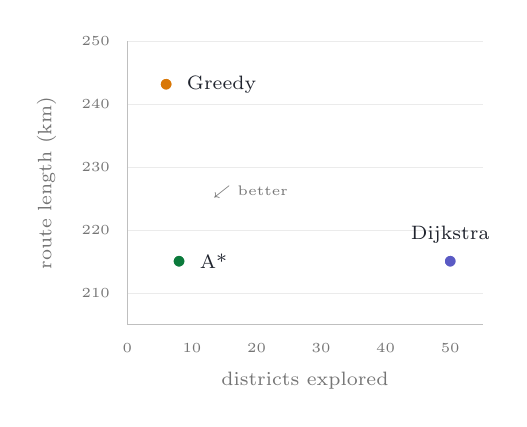
\begin{tikzpicture}[x=0.082cm, y=0.08cm]
    \foreach \v in {210,220,...,250}{%
      \draw[black!8, line width=0.3pt] (0,\v-205) -- (55,\v-205);
      \node[font=\tiny, text=neutralg, anchor=east] at (-1.2,\v-205) {\v};}
    \foreach \v in {0,10,...,50}{%
      \node[font=\tiny, text=neutralg, anchor=north] at (\v,-1.4) {\v};}
    \draw[black!25, line width=0.3pt] (0,0) -- (55,0);
    \draw[black!25, line width=0.3pt] (0,0) -- (0,45);
    \node[font=\scriptsize, text=neutralg, anchor=north] at (27.5,-6)
      {districts explored};
    \node[font=\scriptsize, text=neutralg, rotate=90, anchor=south] at (-9.5,22.5)
      {route length (km)};
    \node[font=\tiny, text=neutralg] at (19,21) {$\swarrow$ better};
    % marks: series colour, 2px white ring; labels in ink beside them
    \fill[rbluemd,  draw=white, line width=0.8pt] (50,10.1) circle (2.4pt);
    \fill[cbOrange, draw=white, line width=0.8pt] (6,38.2)  circle (2.4pt);
    \fill[cbGreen,  draw=white, line width=0.8pt] (8,10.1)  circle (2.4pt);
    \node[font=\scriptsize, text=blkInk, anchor=south, yshift=3pt] at (50,10.1) {Dijkstra};
    \node[font=\scriptsize, text=blkInk, anchor=west,  xshift=4pt] at (6,38.2)  {Greedy};
    \node[font=\scriptsize, text=blkInk, anchor=west,  xshift=4pt] at (8,10.1)  {A*};
  \end{tikzpicture}}

% bars: districts explored, 0-50; <=24px thick, rounded data-end,
% square at the baseline, value at the tip in ink
\newcommand{\cmpbars}{%
  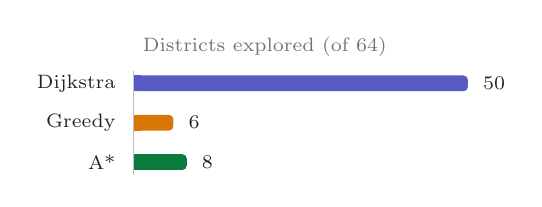
\begin{tikzpicture}[x=0.085cm, y=1cm]
    \node[font=\scriptsize, text=neutralg, anchor=south west] at (0,0.22)
      {Districts explored (of 64)};
    \foreach \y/\c/\nm/\v in {0/rbluemd/Dijkstra/50, -0.5/cbOrange/Greedy/6,
                              -1.0/cbGreen/A*/8}{%
      \fill[\c, rounded corners=1.6pt] (0,\y-0.1) rectangle (\v,\y+0.1);
      \fill[\c] (0,\y-0.1) rectangle (1.2,\y+0.1);
      \node[font=\scriptsize, text=blkInk, anchor=east] at (-1.2,\y) {\nm};
      \node[font=\scriptsize, text=blkInk, anchor=west] at (\v+0.8,\y) {\v};}
    \draw[black!25, line width=0.3pt] (0,0.16) -- (0,-1.16);
  \end{tikzpicture}}

% bars: route length, 0-250 km, a touch shorter than \cmpbars so the
% "243 (+28)" label stays inside the slide; baseline at zero, so the
% gap to optimal is shown honestly.  Dashed rule = shortest route, 215 km.
\newcommand{\cmproute}{%
  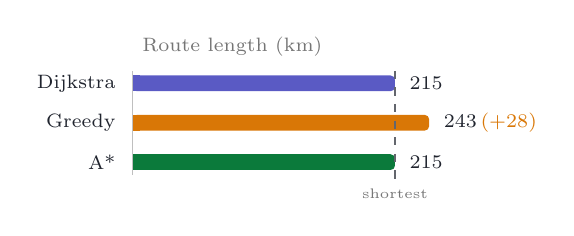
\begin{tikzpicture}[x=0.0155cm, y=1cm]
    \node[font=\scriptsize, text=neutralg, anchor=south west] at (0,0.22)
      {Route length (km)};
    \foreach \y/\c/\nm/\v/\x in {0/rbluemd/Dijkstra/215/,
                                 -0.5/cbOrange/Greedy/243/\,\textcolor{cbOrange}{(+28)},
                                 -1.0/cbGreen/A*/215/}{%
      \fill[\c, rounded corners=1.6pt] (0,\y-0.1) rectangle (\v,\y+0.1);
      \fill[\c] (0,\y-0.1) rectangle (6,\y+0.1);
      \node[font=\scriptsize, text=blkInk, anchor=east] at (-6,\y) {\nm};
      \node[font=\scriptsize, text=blkInk, anchor=west] at (\v+4,\y) {\v\x};}
    \draw[black!25, line width=0.3pt] (0,0.16) -- (0,-1.16);
    \draw[blkInk!70, dashed, line width=0.5pt] (215,0.16) -- (215,-1.22);
    \node[font=\tiny, text=neutralg, anchor=north] at (215,-1.22)
      {shortest};
  \end{tikzpicture}}

% ---------- 11c. three result maps (small multiples) ------------------
%      The same map three times: what each search explored, and the route
%      it returned.  Dots in the plot colours validated above; the static
%      map is already cached by \bdbase, so each panel only adds its dots.
%      ov1 Dijkstra, ov2 Greedy, ov3 A*, ov4 closing line.
\newcommand{\cmpmap}[1]{% #1 = the layer drawn on the base map
  \scalebox{0.8}{%
    \begin{tikzpicture}[x=\bdscalex, y=\bdscaley,
                        shift={(-87.98,-20.75)}, every node/.style={inner sep=0pt}]
      \bdbase #1
    \end{tikzpicture}}}
% Dijkstra: the 49 settled districts + Dhaka = 50, tree edges hidden
\newcommand{\cmpdjlayer}{%
  \begin{scope}[bdtree/.style={draw=none},
                bdclosed/.style={bdcity, fill=rbluemd, minimum size=1.5mm}]
    \bdsettled
  \end{scope}
  \bdroute \bdends}
% Greedy: the 6 districts it expanded are exactly its route
\newcommand{\cmpgrlayer}{\bdgroute \bdends}
% A*: its route (6) + the two it looked at and dropped = 8
\newcommand{\cmpaslayer}{%
  \foreach \n in {gazipur, kishoreganj}
    {\node[bdcity, fill=cbGreen!45, minimum size=1.5mm] at (\n) {};}
  \bdroute \bdends}
% caption under a panel: #1 colour, #2 name, #3 explored, #4 km, #5 verdict
\newcommand{\cmpcap}[5]{%
  {\footnotesize\textcolor{#1}{\textbf{#2}}\par}
  \vspace{1pt}
  {\scriptsize explored \textbf{#3} of 64\\ route #4\,km\quad #5\par}}

% ---------- 11c. three result maps -- switched off --------------------
%      Replaced by the table + bars frame below.  To bring it back, delete
%      the \iffalse / \fi pair around it (and switch the one below off).
\iffalse
\begin{frame}{Dijkstra vs Greedy vs A*}
  \begin{columns}[T]
    \column{0.33\textwidth}
      \centering
      \cmpmap{\cmpdjlayer}\par
      \vspace{0.2em}
      \cmpcap{rbluemd}{Dijkstra}{50}{215}{\pos{$\checkmark$ optimal}}

    \column{0.33\textwidth}
      \centering
      \onslide<2->{%
      \cmpmap{\cmpgrlayer}\par
      \vspace{0.2em}
      \cmpcap{cbOrange}{Greedy}{6}{243}{\bad{$\times$ not optimal}}}

    \column{0.33\textwidth}
      \centering
      \onslide<3->{%
      \cmpmap{\cmpaslayer}\par
      \vspace{0.2em}
      \cmpcap{cbGreen}{A*}{8}{215}{\pos{$\checkmark$ optimal}}}
  \end{columns}

  \vspace{0.6em}
  \onslide<4->{%
  \begin{center}\small
    A* explores almost as little as Greedy, and still returns
    Dijkstra's route.
  \end{center}}
\end{frame}
\fi

% ---------- 11b. table + bars -----------------------------------------
%      Top bars: how much each search looked at.  Bottom bars: how good
%      the route it returned is.
\begin{frame}{Dijkstra vs Greedy vs A*}
  \begin{columns}[c]
  \column{0.5\textwidth}
    \cmptable\par
  \column{0.4\textwidth}
    \centering
    \onslide<2->{\cmpbars}\par
    \vspace{1.4em}
    \onslide<3->{\cmproute}
  \end{columns}
\end{frame}


\begin{frame}{Summary --- Dijkstra vs Greedy vs A*}
  \vspace{6pt}
  \begin{columns}[T]
    \column{0.33\textwidth}
      \centering
      \usebox{\gpdj}\par
      \vspace{0.4em}
      {\footnotesize\textbf{Dijkstra}\\[2pt]
       \onslide<1->{cells: \bad{\statdijkstraexp}\\
                    cost: \pos{\statdijkstrapath}}}

    \column{0.33\textwidth}
      \centering
      \onslide<1->{\usebox{\gpgr}}\par
      \vspace{0.4em}
      {\footnotesize\onslide<1->{\textbf{Greedy}}\\[2pt]
       \onslide<1->{cells: \pos{\statgreedyexp}\\
                    cost: \bad{\statgreedypath}}}

    \column{0.33\textwidth}
      \centering
      \onslide<1->{\usebox{\gpas}}\par
      \vspace{0.4em}
      {\footnotesize\onslide<1->{\textbf{A*}}\\[2pt]
       \onslide<1->{cells: \pos{\statastarexp}\\
                    cost: \pos{\statastarpath}}}
  \end{columns}

  \vspace{0.8em}
  \onslide<2->{%
  \begin{center}\small
    Far fewer expansions than Dijkstra, \emph{and} a provably cheapest
    route --- \HL{that is A*.}
  \end{center}}
\end{frame}

% ---------- SUMMARY, flat 2D (part1 frame 20) -- switched off ----------
%      Replaced by the 3D frame above.  To bring it back, delete the
%      \iffalse / \fi pair around it (and remove the 3D frame).
\iffalse
\begin{frame}{Summary --- Dijkstra vs Greedy vs A*}
  \vspace{9.3pt}
  \begin{columns}[c]
    \column{0.33\textwidth}
      \begin{center}
        \only<1->{\gridpictiny{0.235cm}{grids/mini-dijkstra}}
      \end{center}
      \vspace{0.2em}
      \begin{center}\footnotesize
        \only<1->{\textbf{Dijkstra}\\[2pt]}
        \only<2->{cells: \bad{\statdijkstraexp}\\
                     cost: \pos{\statdijkstrapath}}
      \end{center}

    \column{0.33\textwidth}
      \begin{center}
        \only<3->{\gridpictiny{0.235cm}{grids/mini-greedy}}
      \end{center}
      \vspace{0.2em}
      \begin{center}\footnotesize
        \only<3->{\textbf{Greedy}\\[2pt]}
        \only<4->{cells: \pos{\statgreedyexp}\\
                     cost: \bad{\statgreedypath}}
      \end{center}

    \column{0.33\textwidth}
      \begin{center}
        \only<5->{\gridpictiny{0.235cm}{grids/mini-astar}}
      \end{center}
      \vspace{0.2em}
      \begin{center}\footnotesize
        \only<5->{\textbf{A*}\\[2pt]}
        \only<6->{cells: \pos{\statastarexp}\\
                     cost: \pos{\statastarpath}}
      \end{center}
  \end{columns}

  \vspace{0.8em}
  \only<7->{
  \begin{center}\small
    Far fewer expansions than Dijkstra, \emph{and} a provably cheapest
    route --- \HL{that is A*.}
  \end{center}}
\end{frame}
\fi

\end{document}


% ---------- part 2 
\partsetup{2}
\begin{frame}{Roadmap}\centering\partbanner{2}\end{frame}
% !TEX program = xelatex
\documentclass[aspectratio=169,10pt]{beamer}

\input{preamble2}
\input{part2-defs}          % part 2 macros (also loaded by ../combined.tex)
\newcommand{\statdijkstraexp}{137}
\newcommand{\statdijkstrapath}{19}
\newcommand{\statgreedyexp}{48}
\newcommand{\statgreedypath}{35}
\newcommand{\statastarexp}{81}
\newcommand{\statastarpath}{19}


\begin{document}

% ---------- shared macro: a small labelled grid + a distance readout ---
\newcommand{\distgrid}[3]{%   #1 = draw commands (tikz), #2 = caption, #3 = formula
  \begin{minipage}[t]{4.55cm}
    \centering
    \begin{tikzpicture}[x=0.34cm,y=0.34cm]
      \foreach \c in {0,...,8}{\foreach \r in {0,...,5}{\gcell{gfree}{\c}{\r}}}
      #1
    \end{tikzpicture}\par
    \vspace{2pt}
    {\footnotesize #2}\par
    {\scriptsize\mut{#3}}
  \end{minipage}}

 
% ---------- 11a. what f, g, h are ----------------------------------------
\begin{frame}[label=11a]{Defining parameters}
  \begin{columns}[T,onlytextwidth]
  \column{0.5\textwidth}
    \onslide<2->{%
    \begin{block}{$g(v)$ --- cost so far}
      \small
      The exact cost of the \textbf{best known path} from the start $s$ to $v$.
    \end{block}}
    \vspace{0.5em}
    \onslide<3->{%
    \begin{exampleblock}{$h(v)$ --- cost to go}
      \small
      An \textbf{estimate} of the remaining cost from $v$ to the goal $t$.
    \end{exampleblock}}
    \onslide<4->{%
    \begin{alertblock}{$f(v) = g(v) + h(v)$ --- total estimated cost}
      \small
      \textbf{Best guess} for the cost of the \emph{full} $s \to t$ path if it routes through $v$.
    \end{alertblock}}

  \column{0.4\textwidth}
    \vspace{0.6em}

    \onslide<5->{%
    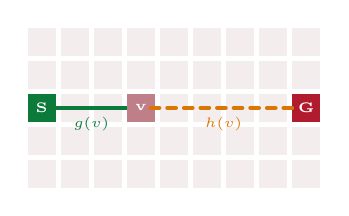
\begin{tikzpicture}[x=0.42cm,y=0.42cm]
      \foreach \c in {0,...,8}{\foreach \r in {0,...,4}{\gcell{gfree}{\c}{\r}}}
      \gletter{gstart}{0}{2}{S}
      \gletter{ggoal}{8}{2}{G}
      \draw[cbGreen, line width=1.6pt, line cap=round]
        (0.7,2.5) -- (3.3,2.5);
      \gletter{gclose}{3}{2}{v}
      \draw[cbOrange, dashed, line width=1.6pt, line cap=round]
      (3.8,2.5) -- (8.2,2.5);
      {\node[font=\tiny, text=cbGreen] at (2,2) {$g(v)$};}
      {\node[font=\tiny, text=cbOrange] at (6,2) {$h(v)$};}
    \end{tikzpicture}\par
    \vspace{4pt}
    {\footnotesize\textcolor{cbGreen}{$g(v)=3$} --- three steps walked}\par
    {\footnotesize\textcolor{cbOrange}{$h(v)=5$} --- five steps remaining}\par
    {\footnotesize $f(v) = g(v) + h(v) = 3 + 5 = 8$}
    }
  \end{columns}
\end{frame}
 
 
% ---------- 12a. why the heuristic helps --------------------------------
\begin{frame}{Why the heuristic helps}
  \begin{columns}[T]
  \column{0.5\textwidth}
    \centering
    \onslide<1->{%
    {\footnotesize\textbf{No heuristic} --- Dijkstra ($h \equiv 0$)}\\[2pt]
    \gridpicsmall{0.34cm}{grids/mini-dijkstra}\par
    {\scriptsize\textcolor{cbRed}{\statdijkstraexp} cells expanded --- \emph{blind} to where the goal is}}

  \column{0.5\textwidth}
    \centering
    \onslide<2->{%
    {\footnotesize\textbf{With a good heuristic} --- A*}\\[2pt]
    \gridpicsmall{0.34cm}{grids/mini-astar}\par
    {\scriptsize\textcolor{cbGreen}{\statastarexp} cells expanded ---
     \emph{biased} toward the goal}}
  \end{columns}

  \vspace{0.6em}
  \onslide<3->{\takeaway{$h$ does not change \emph{what} A* is allowed to
    explore --- it changes the \emph{order}.}}
\end{frame}


% ---------- 3D-a. the heuristic as a landscape -------------------------
\begin{frame}{The heuristic as a landscape}
  \begin{columns}[T]
  \column{0.58\textwidth}
    \centering
    \begin{tikzpicture}
      \begin{axis}[land3d, land view={-32}{34}{0.38}]
        % the flat map, left on the floor
        \floorA
        % the same map, every node lifted to height h(v)
        \addplot3[tilesurf, colormap name=hblue, samples=13, samples y=13,
                  domain=0:12, y domain=0:12]
          {\kA*veclen(x-\gAx, y-\gAy)};
        % height dimension at the near corner
        \draw[neutralg, line width=0.6pt, {Bar[width=1.6mm]}-{Bar[width=1.6mm]}]
          (12,0,0) -- \liftA{12}{0}
          node[tagbox, text=neutralg, midway, left=2pt] {$h(v)$};
        % the route, rolling downhill
        \draw[edgpath, line cap=round, line join=round, visible on=<2->]
          \liftA{2}{10} -- \liftA{3}{9} -- \liftA{4}{8} -- \liftA{5}{7}
          -- \liftA{6}{6} -- \liftA{7}{5} -- \liftA{7}{4} -- \liftA{7}{3};
        % one step the wrong way
        \draw[move3d,cbRed, visible on=<3->] \liftA{2}{10} -- \liftA{1}{11};
        \node[tagbox, text=cbRed, above=3pt, visible on=<3->]
          at \liftA{1}{11} {uphill: $\Delta f=+2$};
        \node[tagbox, text=cbGreen, left=5pt, visible on=<3->]
          at \liftA{4}{8} {downhill: $\Delta f=0$};
        \node[sball] at \liftA{2}{10} {};
        \node[tag, text=gstart, below left=3pt] at \liftA{2}{10} {\textbf{S}};
        \node[gball] at \liftA{7}{3} {};
        \node[tag, text=ggoal, below=6pt] at \liftA{7}{3} {\textbf{G} \ $h=0$};
      \end{axis}
    \end{tikzpicture}

  \column{0.42\textwidth}
    \begin{block}{Lift the map by $h$}
      \small
      \begin{itemize}\setlength{\itemsep}{5pt}
        \item<1-> raise every node $v$ to height $h(v)$
        \item<1-> $h(G)=0$
        \item<2-> each step costs $+1$ in $g$
        \item<3-> a \pos{downhill} step is incentivized
        \item<3-> an \bad{uphill} step is penalized
      \end{itemize}
    \end{block}
  \end{columns}
\end{frame}


% ---------- 12b. heuristic choice, expanded ---------------------------
\begin{frame}[label=12b]{Choosing a heuristic for A*}
  \begin{columns}[T]
  \column{0.52\textwidth}
    \begin{block}{What $h(v)$ has to be}
      \small
      \begin{itemize}\setlength{\itemsep}{7pt}
        \item<2-> Cheap to compute
        \item<3-> \textbf{Never an overestimate}
        \item<4-> Ideally close to the true remaining cost
      \end{itemize}
    \end{block}

  \column{0.48\textwidth}
    \onslide<5->{%
    \begin{exampleblock}{Common choices}
      \small
      \begin{itemize}\setlength{\itemsep}{6pt}
        \item<5-> Manhattan distance
        \item<5-> Euclidean distance
      \end{itemize}
    \end{exampleblock}}
  \end{columns}
\end{frame}

% ---------- 12c. Manhattan vs Euclidean, diagrams ----------------------
\begin{frame}{Manhattan vs Euclidean distance}
  \centering
  \begin{columns}[T]
  \column{0.5\textwidth}
    \centering
    \onslide<1->{%
    \distgrid{%
      \gletter{gstart}{1}{1}{A}%
      \gletter{ggoal}{6}{4}{B}%
      \onslide<1->{\draw[cbOrange, line width=1.6pt, line cap=round]
        (1.8,1.5) -- (6.5,1.5);}%
      \onslide<1->{\draw[cbOrange, line width=1.6pt, line cap=round]
        (6.5,1.5) -- (6.5,4.2);}%
      \onslide<1->{\node[font=\tiny, text=cbOrange] at (4.0,1.0) {5};}%
      \onslide<1->{\node[font=\tiny, text=cbOrange] at (6.9,3.0) {3};}%
    }{\textbf{Manhattan} \\ $|x_A - x_B| + |y_A - y_B|$}
     {only horizontal / vertical steps --- $5+3=8$}}
  \column{0.5\textwidth}
    \centering
    \onslide<2->{%
    \distgrid{%
      \gletter{gstart}{1}{1}{A}%
      \gletter{ggoal}{6}{4}{B}%
      \draw[rblue, line width=1.6pt, line cap=round] (1.7,1.7) -- (6.3,4.3);
      \node[font=\tiny, text=rblue] at (4.7,2.7) {5.8};
    }{\textbf{Euclidean} \\ $\sqrt{(x_A-x_B)^2+(y_A-y_B)^2}$}
     {any-angle movement --- $\sqrt{5^2+3^2}\approx 5.8$}}
  \end{columns}
\end{frame}

% ---------- 3D-d. Euclidean vs Manhattan in 3D ---------------------------
\begin{frame}{Euclidean vs Manhattan --- in three dimensions}
  \begin{columns}[T]
  \column{0.55\textwidth}
    \centering
    \begin{tikzpicture}[x={(1.22cm,0cm)}, y={(0.66cm,0.48cm)},
                        z={(0cm,1.22cm)}, line join=round, line cap=round]
      % faint cell lattice on the floor
      \foreach \i in {0,...,4}{\draw[gridgray, line width=0.4pt] (\i,0,0) -- (\i,3,0);}
      \foreach \j in {0,...,3}{\draw[gridgray, line width=0.4pt] (0,\j,0) -- (4,\j,0);}
      % the hidden edge
      \draw[gridgray, dashed, line width=0.6pt] (0,3,0) -- (0,3,2);
      % Pythagoras triangle (floor diagonal, rise, space diagonal)
      \fill[rbluelt, opacity=0.8, visible on=<2->] (0,0,0) -- (4,3,0) -- (4,3,2) -- cycle;
      \draw[rbluemd, dashed, line width=1pt, visible on=<2->] (0,0,0) -- (4,3,0)
        node[pos=0.6, below right=-1pt, tag, text=rbluemd] {$5$};
      % the box
      \fill[rbluelt, opacity=0.35] (0,0,2) -- (4,0,2) -- (4,3,2) -- (0,3,2) -- cycle;
      \draw[rbluedk!70, line width=0.8pt]
        (0,0,0) -- (4,0,0) -- (4,0,2) -- (0,0,2) -- cycle
        (4,0,0) -- (4,3,0) -- (4,3,2) -- (4,0,2)
        (0,0,2) -- (0,3,2) -- (4,3,2);
      % Manhattan: one axis at a time, along the edges
      \draw[cbOrange, line width=2.2pt, visible on=<1->]
        (0,0,0) -- (4,0,0) -- (4,3,0) -- (4,3,2);
      \node[tag, text=cbOrange, below=3pt, visible on=<1->] at (2,0,0) {$\Delta x = 4$};
      \node[tag, text=cbOrange, below right=0pt, visible on=<1->] at (4,1.5,0) {$\Delta y = 3$};
      \node[tagbox, text=cbOrange, left=3pt, visible on=<1->] at (4,3,1) {$\Delta z = 2$};
      % Euclidean: straight through the box
      \draw[rblue, line width=2.2pt, visible on=<2->] (0,0,0) -- (4,3,2);
      \node[tagbox, text=rblue, above left=0pt, visible on=<2->] at (2,1.5,1)
        {$\sqrt{29}\approx 5.39$};
      % endpoints
      \node[sball] at (0,0,0) {};
      \node[tag, text=gstart, left=6pt] at (0,0,0) {\textbf{A}};
      \node[gball] at (4,3,2) {};
      \node[tag, text=ggoal, above=6pt] at (4,3,2) {\textbf{B}};
    \end{tikzpicture}

  \column{0.45\textwidth}
    \onslide<1->{%
    \begin{block}{\textcolor{cbOrange}{Manhattan} --- along the edges}
      \small
      $|\Delta x|+|\Delta y|+|\Delta z| = 4+3+2 = \mathbf{9}$\\[2pt]
      {\footnotesize one axis at a time, like a 6-directional grid}
    \end{block}}
    \onslide<2->{%
    \begin{block}{\textcolor{rblue}{Euclidean} --- straight through}
      \small
      $\sqrt{\Delta x^2+\Delta y^2+\Delta z^2} = \sqrt{29} \approx \mathbf{5.39}$\\[2pt]
      {\footnotesize any-angle movement}
    \end{block}}
    \vspace{0.3em}
    \vspace{0.3em}
    \onslide<3->{{\footnotesize Manhattan is \textcolor{cbRed}{never smaller}, equal only
      when $A$ and $B$ differ along a single axis.}}
  \end{columns}
\end{frame}


% ---------- 12d. pseudocode for A* --------------------------------------
\begin{frame}[t]{A* --- pseudocode}
  \begin{columns}[T]

    \column{0.55\textwidth}
    \begin{clrs}[\footnotesize]
      \aline[1-]{\proc{A-Star}$(G, s, t, h)$}
      \aline[1-]{\idt1 \kw{for each} $v \in V$: \
        $g[v] \gets \infty$,\; $\pi[v] \gets \textsc{nil}$}
      \aline[1-]{\idt1 $g[s] \gets 0$}
      \aline[1-]{\idt1 \hlonc{2}{$Q \gets$ priority queue keyed by
        \textcolor{cbGreen}{$g$}$+$\textcolor{cbOrange}{$h$}, holding
        $\{s\}$}}
      \aline[1-]{\idt1 $\mathit{S} \gets \varnothing$}
      \aline[1-]{\idt1 \kw{while} $Q \neq \varnothing$}
      \aline[1-]{\idt2 $u \gets \textsc{Extract-Min}(Q)$}
      \aline[1-]{\idt2 \kw{if} $u = t$:}
      \aline[1-]{\idt3 \kw{return} \proc{Reconstruct}$(\pi, t)$}
      \aline[1-]{\idt2 $\mathit{S} \gets \mathit{S} \cup \{u\}$}
      \aline[1-]{\idt2 \kw{for each} $v$ adjacent to $u$}
      \aline[1-]{\idt3 \kw{if} $v \in \mathit{S}$: \ \kw{continue}}
      \aline[1-]{\idt3 \kw{if} $g[u] + w(u,v) < g[v]$}
      \aline[1-]{\idt4 $g[v] \gets g[u] + w(u,v)$,\; $\pi[v] \gets u$}
      \aline[1-]{\idt4 \hlonc{2}{\textsc{Insert-or-Decrease-Key}
        $\big(Q, v, g[v]+h(v)\big)$}}
    \end{clrs}

    \column{0.45\textwidth}
    \onslide<2->{%
    \begin{block}{Only one difference from Dijkstra}
      \small The priority key changes from $g$ to $(g+h)$. Everywhere
      else, the algorithm is untouched.
    \end{block}}
  \end{columns}
\end{frame}

% ---------- 12e. time complexity, annotated pseudocode ---------------------
\begin{frame}[t, label=12e]{Time complexity analysis}
  \begin{columns}[T]

    \column{0.55\textwidth}
    \begin{clrs}[\footnotesize]
      \aline[1-]{\proc{A-Star}$(G, s, t, h)$}
      \aline[1-]{\idt1 \hlonc{2}{\kw{for each} $v \in V$: \
        $g[v] \gets \infty$,\; $\pi[v] \gets \textsc{nil}$}}
      \aline[1-]{\idt1 $g[s] \gets 0$}
      \aline[1-]{\idt1 $Q \gets$ priority queue keyed by $g+h$, holding
        $\{s\}$}
      \aline[1-]{\idt1 $\mathit{S} \gets \varnothing$}
      \aline[1-]{\idt1 \hlonc{3}{\kw{while} $Q \neq \varnothing$}}
      \aline[1-]{\idt2 \hlonc{3}{$u \gets \textsc{Extract-Min}(Q)$}}
      \aline[1-]{\idt2 \kw{if} $u = t$:}
      \aline[1-]{\idt3 \kw{return} \proc{Reconstruct}$(\pi, t)$}
      \aline[1-]{\idt2 $\mathit{S} \gets \mathit{S} \cup \{u\}$}
      \aline[1-]{\idt2 \hlonc{4}{\kw{for each} $v$ adjacent to $u$}}
      \aline[1-]{\idt3 \kw{if} $v \in \mathit{S}$: \ \kw{continue}}
      \aline[1-]{\idt3 \kw{if} $g[u] + w(u,v) < g[v]$}
      \aline[1-]{\idt4 $g[v] \gets g[u] + w(u,v)$,\;
        $\pi[v] \gets u$}
      \aline[1-]{\idt4 \hlonc{5}{\textsc{Insert-or-Decrease-Key}
        $\big(Q, v, g[v]+h(v)\big)$}}
    \end{clrs}

    \column{0.45\textwidth}
    \onslide<2->{%
    \begin{exampleblock}{\textcolor{cbOrange}{Init}}
      \scriptsize $O(|V|)$ for touching every vertex once
    \end{exampleblock}
    \vspace{0.2em}
    \begin{exampleblock}{\textcolor{cbGreen}{Main loop}}
      \scriptsize $O(|V|\log|V|)$ on a binary heap
    \end{exampleblock}
    \vspace{0.2em}
    \begin{exampleblock}{\textcolor{rblue}{Edge scan}}
      \scriptsize $O(|E|)$ for considering every edge
    \end{exampleblock}
    \vspace{0.2em}
    \begin{alertblock}{\textcolor{cbRed}{Heap update}}
      \scriptsize $O(\log|V|)$ each, up to $O(|E|\log|V|)$ total
    \end{alertblock}}
  \end{columns}
\end{frame}

% ---------- 12e-2. time complexity, the sum -------------------------------
\begin{frame}[label=12e2]{Time complexity --- putting it together}
  % \small
  \begin{itemize}\setlength{\itemsep}{9pt}
    \item<1-> \textbf{\textcolor{cbOrange}{Initialization}}: $O(|V|)$
    \item<2-> \textbf{\textcolor{cbGreen}{Extractions}}: $O(|V|\log|V|)$
    \item<3-> \textbf{\textcolor{rblue}{Edge scans}}: $O(|E|)$
    \item<4-> \textbf{\textcolor{cbRed}{Heap insert / decrease-key}}: $O(|E|\log|V|)$
  \end{itemize}

  \vspace{0.6em}
  \onslide<5->{%
  \[
    O(|V|) + O(|V|\log|V|) + O(|E|) + O(|E|\log|V|)
  \]}
  \onslide<6->{%
  \begin{center}
    \Large\(\Rightarrow\quad
    \boxed{O\big((|V|+|E|)\log |V|\big)}\)
  \end{center}}
\end{frame}

% ---------- 12e-3. space complexity, annotated pseudocode ------------------
\begin{frame}[t, label=12e3]{Space complexity analysis}
  \begin{columns}[T]

    \column{0.55\textwidth}
    \begin{clrs}[\footnotesize]
      \aline[1-]{\proc{A-Star}$(G, s, t, h)$}
      \aline[1-]{\idt1 \hlonc{2}{\kw{for each} $v \in V$: \
        $g[v] \gets \infty$,\; $\pi[v] \gets \textsc{nil}$}}
      \aline[1-]{\idt1 $g[s] \gets 0$}
      \aline[1-]{\idt1 \hlonc{3}{$Q \gets$ priority queue keyed by
        $g+h$, holding $\{s\}$}}
      \aline[1-]{\idt1 \hlonc{3}{$\mathit{S} \gets \varnothing$}}
      \aline[1-]{\idt1 \kw{while} $Q \neq \varnothing$}
      \aline[1-]{\idt2 $u \gets \textsc{Extract-Min}(Q)$}
      \aline[1-]{\idt2 \kw{if} $u = t$:}
      \aline[1-]{\idt3 \hlonc{4}{\kw{return} \proc{Reconstruct}$(\pi, t)$}}
      \aline[1-]{\idt2 \hlonc{3}{$\mathit{S} \gets \mathit{S} \cup \{u\}$}}
      \aline[1-]{\idt2 \hlonc{3}{\kw{for each} $v$ adjacent to $u$}}
      \aline[1-]{\idt3 \kw{if} $v \in \mathit{S}$: \ \kw{continue}}
      \aline[1-]{\idt3 \kw{if} $g[u] + w(u,v) < g[v]$}
      \aline[1-]{\idt4 \hlonc{3}{$g[v] \gets g[u] + w(u,v)$,\;
        $\pi[v] \gets u$}}
      \aline[1-]{\idt4 \hlonc{3}{\textsc{Insert-or-Decrease-Key}
        $\big(Q, v, g[v]+h(v)\big)$}}
    \end{clrs}

    \column{0.45\textwidth}
    \onslide<2->{%
    \begin{exampleblock}{\textcolor{cbOrange}{$g$ and $\pi$ arrays}}
      \scriptsize One entry per vertex: $O(|V|)$
    \end{exampleblock}
    \vspace{0.4em}
    \begin{exampleblock}{\textcolor{cbGreen}{Frontier $Q$ and closed set $S$}}
      \scriptsize Every vertex is generated at most once: together $O(|V|)$.
    \end{exampleblock}
    \vspace{0.4em}
    \begin{alertblock}{\textcolor{rblue}{Reconstructed path}}
      \scriptsize $O(|V|)$ as typically $O(d) \ll |V|$
    \end{alertblock}}
  \end{columns}
\end{frame}

% ---------- 12e-4. space complexity, the sum --------------------------------
\begin{frame}[label=12e4]{Space complexity --- putting it together}
  \small
  \begin{itemize}\setlength{\itemsep}{9pt}
    \item<1-> \textbf{\textcolor{cbOrange}{$g[\cdot]$ and
          $\pi[\cdot]$}}: $O(|V|)$
    \item<2-> \textbf{\textcolor{cbGreen}{Priority queue $Q$ and
          closed set $\mathit{S}$}}: $O(|V|)$
    \item<3-> \textbf{\textcolor{rblue}{Path reconstruction}}: $O(|V|)$ worst case
  \end{itemize}

  \vspace{0.6em}
  \onslide<4->{%
  \[
    O(|V|) + O(|V|) + O(|V|)
  \]}
  \onslide<5->{%
  \begin{center}
    \Large\(\Rightarrow\quad \boxed{O(|V|)}\)
  \end{center}}
  \onslide<6->{%
  \begin{center}
    \mut{No dependence on $|E|$.} }
  \end{center}
\end{frame}

% ---------- 12f. complexity comparison table -----------------------------
\begin{frame}[label=12f]{Complexity, side by side}
  \centering
  {\footnotesize
  \renewcommand{\arraystretch}{1.18}
  \begin{tabular}{@{}l@{\hspace{1.4em}}c@{\hspace{1.4em}}c@{\hspace{1.4em}}c@{}}
    \toprule
     & \textcolor{rbluemd}{\shortstack{\textbf{Dijkstra}}} & \textcolor{cbOrange}{\shortstack{\textbf{Greedy}}}
     & \textcolor{cbGreen}{\shortstack{\textbf{A*}}}\\
    \midrule
    {\shortstack[l]{Time (worst case)}}
      & {$O((|V|{+}|E|)\log|V|)$}
      & {$O((|V|{+}|E|)\log|V|)$}
      & {$O((|V|{+}|E|)\log|V|)$}\\[5pt]
    {Space}
      & {$O(|V|)$} & {$O(|V|)$} & {$O(|V|)$}\\[3pt]
    {\shortstack[l]{Nodes expanded}}
      & {most / all} & {few, unpredictable}
      & {few, provably safe}\\[5pt]
    {Optimal?}
      & {\textcolor{cbGreen}{$\checkmark$}} & {\textcolor{cbRed}{$\times$}}
      & {\textcolor{cbGreen}{$\checkmark$}}\\
    \bottomrule
  \end{tabular}\par}

  \vspace{0.8em}
  \onslide<2->{\begin{center}\footnotesize\mut{Same asymptotic worst
    case as Dijkstra --- A* wins in \emph{practice}, not in the
    textbook bound.}\end{center}}
\end{frame}

\begin{frame}[label=12g0]{Correctness conditions}
  \begin{center}
  
\begin{tikzpicture}
    \node<1->[draw=rblue, fill=rbluelt, rounded corners=3pt, line width=1pt,
        text width=4.8cm, align=center, inner sep=12pt] at (0,0)
      {{\small\mut{1}}\\[3pt]{\bfseries\large\HL{Admissibility}}};
    \node<2->[draw=cbOrange, fill=cbOrangeLt, rounded corners=3pt,
        line width=1pt, text width=4.8cm, align=center, inner sep=12pt]
        at (6.2,0)
      {{\small\mut{2}}\\[3pt]{\bfseries\large\con{Consistency}}};
  \end{tikzpicture}
  \end{center}
\end{frame}

% ---------- 12g. admissibility ------------------------------------------
\begin{frame}[label=12g]{Correctness --- admissibility}
  \begin{columns}[T]
  \column{0.55\textwidth}
    \begin{block}{Definition}
      \small A heuristic $h$ is \textbf{admissible} if, for every node
      $v$,
      \[ h(v) \;\le\; h^{*}(v) \]
      where $h^{*}(v)$ is the \emph{true} cheapest cost from $v$ to the
      goal.
    \end{block}
    \vspace{0.6em}
    \onslide<2->{%
    \begin{exampleblock}{Why it guarantees optimality}
      \small When A* pops $t$, every other node in $Q$ has
      $f = g+h \ge$ that $f$-value. Since $h$ never overestimates,
      nothing left in the queue can beat $t$'s true cost.
    \end{exampleblock}}

  \column{0.45\textwidth}
    \onslide<2->{%
    \centering
    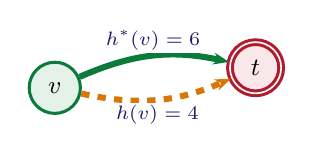
\begin{tikzpicture}[x=0.85cm,y=0.85cm]
      \node[vstart] (v) at (0,0) {$v$};
      \node[vgoal]  (t) at (3,0.3) {$t$};
      \draw[edgpath, {Stealth[length=2mm]}-, -{Stealth[length=2mm]}]
        (v) to[bend left=18] node[wlab, above] {$h^{*}(v)=6$} (t);
      \draw[edgorange, dashed, -{Stealth[length=2mm]}]
        (v) to[bend right=18] node[wlab, below] {$h(v)=4$} (t);
    \end{tikzpicture}\par
    {\footnotesize\textcolor{cbGreen}{$h(v)=4 \le h^{*}(v)=6$} ---
     admissible}\par
    \vspace{4pt}
    {\footnotesize\textcolor{cbRed}{if instead $h(v)=8$} --- not
     admissible}}
  \end{columns}
\end{frame}

% ---------- 12h. consistency --------------------------------------------
\begin{frame}[label=12h]{Correctness --- consistency}
  \begin{columns}[T]
  \column{0.55\textwidth}
    \begin{block}{Definition}
      \small A heuristic $h$ is \textbf{consistent} if, for
      every edge $(u,v)$ with weight $w(u,v)$,
      \[ h(u) \;\le\; w(u,v) + h(v) \]
      with $h(\text{goal})=0$.
    \end{block}
    \vspace{0.6em}
    \onslide<2->{%
    \begin{exampleblock}{Why it matters}
      \small The \textbf{triangle inequality} applied to $h$: \\ $f=g+h$ never
      decreases along a path.
    \end{exampleblock}}

  \column{0.45\textwidth}
    \onslide<2->{%
    \centering
    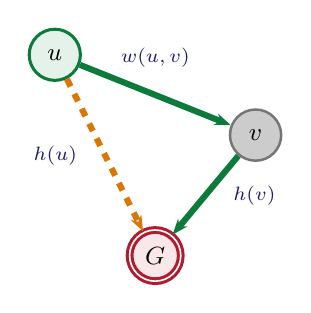
\begin{tikzpicture}[x=0.85cm,y=0.85cm]
      \node[vstart] (u) at (0,1.2)  {$u$};
      \node[vclosed]  (v) at (3,0)    {$v$};
      \node[vgoal]  (t) at (1.5,-1.8) {$G$};

      \draw[edgpath, -{Stealth[length=2mm]}]
        (u) -- node[wlab, above, yshift=8pt] {$w(u,v)$} (v);
      \draw[edgpath, -{Stealth[length=2mm]}]
        (v) -- node[wlab, right, xshift=8pt] {$h(v)$} (t);
      \draw[edgorange, dashed, -{Stealth[length=2mm]}]
        (u) -- node[wlab, left, xshift=-8pt] {$h(u)$} (t);
    \end{tikzpicture}\par
    {\footnotesize \mut{$h(u) \le w(u,v) + h(v)$ --- the triangle inequality in effect.}}}

  \end{columns}
\end{frame}

% ---------- 12j. a bad heuristic, worked examples (expanded, animated) ---
\begin{frame}{A bad heuristic (I) --- overestimating}
  \centering
  {\footnotesize\textbf{Overestimating $h$} --- looks like Greedy}\\[4pt]
  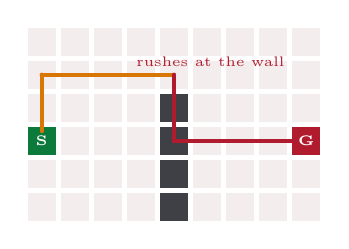
\begin{tikzpicture}[x=0.42cm,y=0.42cm]
    \onslide<1->{%
    \foreach \c in {0,...,8}{\foreach \r in {0,...,5}{\gcell{gfree}{\c}{\r}}}
    \foreach \r in {0,1,2,3}{\gcell{gwall}{4}{\r}}
    \gletter{gstart}{0}{2}{S}
    \gletter{ggoal}{8}{2}{G}}
    \onslide<2->{\draw[cbOrange, line width=1.6pt, line cap=round]
      (0.5,2.8) -- (0.5,4.5);}
    \onslide<3->{\draw[cbOrange, line width=1.6pt, line cap=round]
      (0.5,4.5) -- (4.5,4.5);}
    \onslide<4->{\draw[cbRed, line width=1.6pt, line cap=round]
      (4.5,4.5) -- (4.5,2.5);
      \node[font=\tiny, text=cbRed] at (5.6,4.9) {rushes at the wall};}
    \onslide<5->{\draw[cbRed, line width=1.6pt, line cap=round]
      (4.5,2.5) -- (8.2,2.5);}
  \end{tikzpicture}\par
  \vspace{2pt}
  \begin{itemize}
    \item<5-> \footnotesize Inadmissible
    \item<5-> \footnotesize Behaves like Greedy
    \item<5-> \footnotesize \textcolor{cbRed}{Can return a longer-than-optimal path}
  \end{itemize}
\end{frame}

% ---------- 12j-2. uninformative heuristic --------------------------------
\begin{frame}{A bad heuristic (II) --- uninformative}
  \centering
  {\footnotesize\textbf{Uninformative $h$} --- looks like Dijkstra}\\[4pt]
  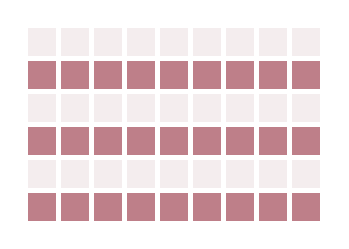
\begin{tikzpicture}[x=0.42cm,y=0.42cm]
    \onslide<1->{%
    \foreach \c in {0,...,8}{\foreach \r in {0,...,5}{\gcell{gfree}{\c}{\r}}}
    \gletter{gstart}{0}{2}{S}
    \gletter{ggoal}{8}{2}{G}}
    \onslide<2->{\foreach \c in {0,1,2}{\foreach \r in {0,2,4}{\gcell{gclose}{\c}{\r}}}}
    \onslide<3->{\foreach \c in {3,4,5}{\foreach \r in {0,2,4}{\gcell{gclose}{\c}{\r}}}}
    \onslide<4->{\foreach \c in {6,7,8}{\foreach \r in {0,2,4}{\gcell{gclose}{\c}{\r}}}}
  \end{tikzpicture}\par
  \vspace{2pt}
  \begin{itemize}
    \item<4-> \footnotesize $h(v)=1$ for all non-goal $v$
    \item<4-> \footnotesize \textbf{Admissible}, but slow --- same as Dijkstra
  \end{itemize}
\end{frame}

% ---------- 12j-3. admissible but locally misleading ----------------------
\begin{frame}{A bad heuristic (III) --- admissible but misleading}
  \centering
  {\footnotesize\textbf{Admissible $h$, dead-end pocket} --- correct,
   yet still wasteful}\\[4pt]
   \vspace{0.6em}
  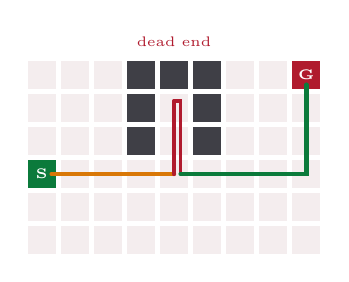
\begin{tikzpicture}[x=0.42cm,y=0.42cm]
    \onslide<1->{%
    \foreach \c in {0,...,8}{\foreach \r in {0,...,5}{\gcell{gfree}{\c}{\r}}}
    \foreach \r in {3,4,5}{\gcell{gwall}{3}{\r}}
    \foreach \r in {3,4,5}{\gcell{gwall}{5}{\r}}
    \gcell{gwall}{4}{5}
    \gletter{gstart}{0}{2}{S}
    \gletter{ggoal}{8}{5}{G}}
    \onslide<2->{\draw[cbOrange, line width=1.6pt, line cap=round]
      (0.8,2.5) -- (4.5,2.5);}
    \onslide<3->{\draw[cbRed, line width=1.6pt, line cap=round]
      (4.5,2.5) -- (4.5,4.7);
      \node[font=\tiny, text=cbRed] at (4.5,6.5) {dead end};}
    \onslide<4->{\draw[cbRed, line width=1.3pt, line cap=round]
      (4.5, 4.7) -- (4.7,4.7) -- (4.7,2.5);}
    \onslide<5->{\draw[cbGreen, line width=1.6pt, line cap=round]
      (4.7,2.5) -- (8.5,2.5) -- (8.5,5.2);}
  \end{tikzpicture}\par
  \vspace{2pt}
  \begin{itemize}
    \item<5-> \footnotesize Still \textbf{admissible} --- just blind to the obstacle
    \item<5-> \footnotesize \bad{Finds the optimal path, but wastes a detour} on a dead end
  \end{itemize}
\end{frame}

% ---------- 12j-4. three failure modes, side by side -----------------------
\begin{frame}[label=12j4]{Three ways a heuristic can go wrong}
  \centering
  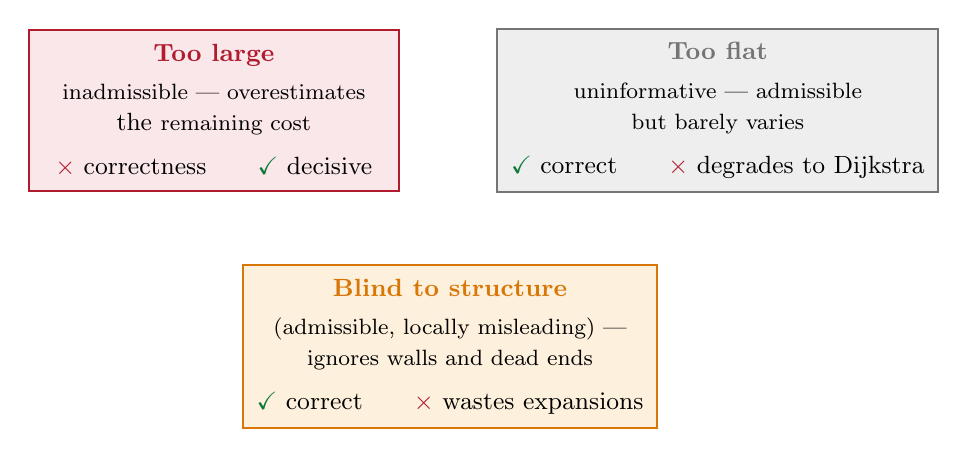
\begin{tikzpicture}[
      algbox/.style = {draw, line width=0.8pt, align=center, font=\small,
                       minimum width=4.7cm, minimum height=1.85cm, inner sep=5pt},
      flow/.style   = {-{Stealth[length=2.4mm]}, line width=1.0pt, draw=neutralg},
      flowlab/.style= {font=\footnotesize, text=neutralg, inner sep=2pt}]

    \node<2->[algbox, draw=cbRed, fill=cbRedLt] (large) at (-4.2,2)
      {\textcolor{cbRed}{\textbf{Too large}}\\[3pt]
       \footnotesize inadmissible --- overestimates \\ the \footnotesize remaining cost \\[5pt]
       \textcolor{cbRed}{$\times$}~correctness\qquad
       \textcolor{cbGreen}{$\checkmark$}~decisive};

    \node<3->[algbox, draw=neutralg, fill=neutralg!12] (flat) at (2.2,2)
      {\textcolor{neutralg}{\textbf{Too flat}}\\[3pt]
       \footnotesize uninformative --- admissible \\ \footnotesize but barely varies \\[5pt]
       \textcolor{cbGreen}{$\checkmark$}~correct\qquad
       \textcolor{cbRed}{$\times$}~degrades to Dijkstra};

    \node<4->[algbox, draw=cbOrange, fill=cbOrangeLt] (blind) at (-1.2,-1)
      {\textcolor{cbOrange}{\textbf{Blind to structure}}\\[3pt]
       \footnotesize (admissible, locally misleading) --- \\
       \footnotesize ignores walls and dead ends\\[5pt]
       \textcolor{cbGreen}{$\checkmark$}~correct\qquad
       \textcolor{cbRed}{$\times$}~wastes expansions};

  \end{tikzpicture}
\end{frame}

\end{document}

% ---------- part 3 
\partsetup{3}
\begin{frame}{Roadmap}\centering\partbanner{3}\end{frame}
% !TEX program = xelatex
% Compile from this directory with XeLaTeX, twice.
% fix-cm has to come before the class; combined.tex loads it itself
\ifdefined\combineddeck\else\RequirePackage{fix-cm}\fi
\documentclass[aspectratio=169,10pt]{beamer}
\input{setup}
\begin{document}

\begin{frame}{We know A*. Now, a trip to Sylhet.}
  \foreach \s in {1,...,5}{\only<\s>{\IntroScene{\s}}}
\end{frame}

\begin{frame}{\StateHeading{\StoryBeatsOne}}
  \StorySequence{\StoryBeatsOne}
\end{frame}

\begin{frame}{\StateHeading{\StoryBeatsTwo}}
  \StorySequence{\StoryBeatsTwo}
\end{frame}

\begin{frame}{\StateHeading{\StoryBeatsThree}}
  \StorySequence{\StoryBeatsThree}
\end{frame}

\begin{frame}{A new question about the heuristic}
  \foreach \s in {1,2}{\only<\s>{\HeuristicQuestionScene{\s}}}
\end{frame}

\begin{frame}{\OptimalityHeading}
  \foreach \s [count=\beat] in {4,5,8,10,13,14,15}{\only<\beat>{\OptimalityScene{\s}}}
\end{frame}

\begin{frame}{A good estimate stays within the truth}
  \foreach \s in {1,...,3}{\only<\s>{\AdmissibilityScene{\s}}}
\end{frame}

\begin{frame}{\HeuristicBridgeHeading}
  % State 1 is the bare seam page, deliberately skipped: the frame opens with the
  % markers already placed. The axis still matches page 28 pixel for pixel.
  \foreach \s [count=\beat] in {2,3}{\only<\beat>{\HeuristicBridgeScene{\s}}}
\end{frame}

\begin{frame}{The beauty of A*}
  \foreach \s in {1,...,3}{\only<\s>{\ClosingScene{\s}}}
\end{frame}

\begin{frame}{A* in action}
  \ThankYouScene
\end{frame}

\end{document}


\end{document}
